\documentclass[dvipdfmx]{beamer}
%テーマ
\usetheme[numbering=counter,shape=pentagon]{LightTheme}
%パッケージ
\usepackage{pxjahyper}
\usepackage{tikz}
\usepackage[absolute,overlay]{textpos}
\usepackage{xcolor}
%tikzライブラリ
\usetikzlibrary{arrows.meta}
\usetikzlibrary{positioning}
\usetikzlibrary{shapes.callouts}
%フォント
\renewcommand{\kanjifamilydefault}{\gtdefault}

%タイトル設定
\title{TechRingにかける想い}
\subtitle{学科を超えて}
\author[Jin]{石田 優仁}
\institute[TechRing]{奈良高専TechRing}
\date[2023/04/30]{2023/04/30}

\begin{document}

\begin{frame}[plain,noframenumbering]
  \begin{flushright}
      \includegraphics[width=2.3cm]{pic/Logo.png}
  \end{flushright}
  \titlepage
\end{frame}

\begin{frame}{高専どんなところ?}

  \begin{block}{国立高等専門学校の特徴}
    \begin{itemize}
      \setlength{\itemsep}{1mm}
      \item 5年制、一貫のカリキュラム
      \item 電気電子系や機械系に限らず、物質や建築、商船もある
      \item \alert{高専祭}という文化祭での文化発表が活発
      \item \alert{ロボコン}やデザコン、プロコンなどのコンテストが充実
      \item \alert{高専カンファレンス}や様々な技術コミュニティでの交流
    \end{itemize}
  \end{block}

  \begin{center}
    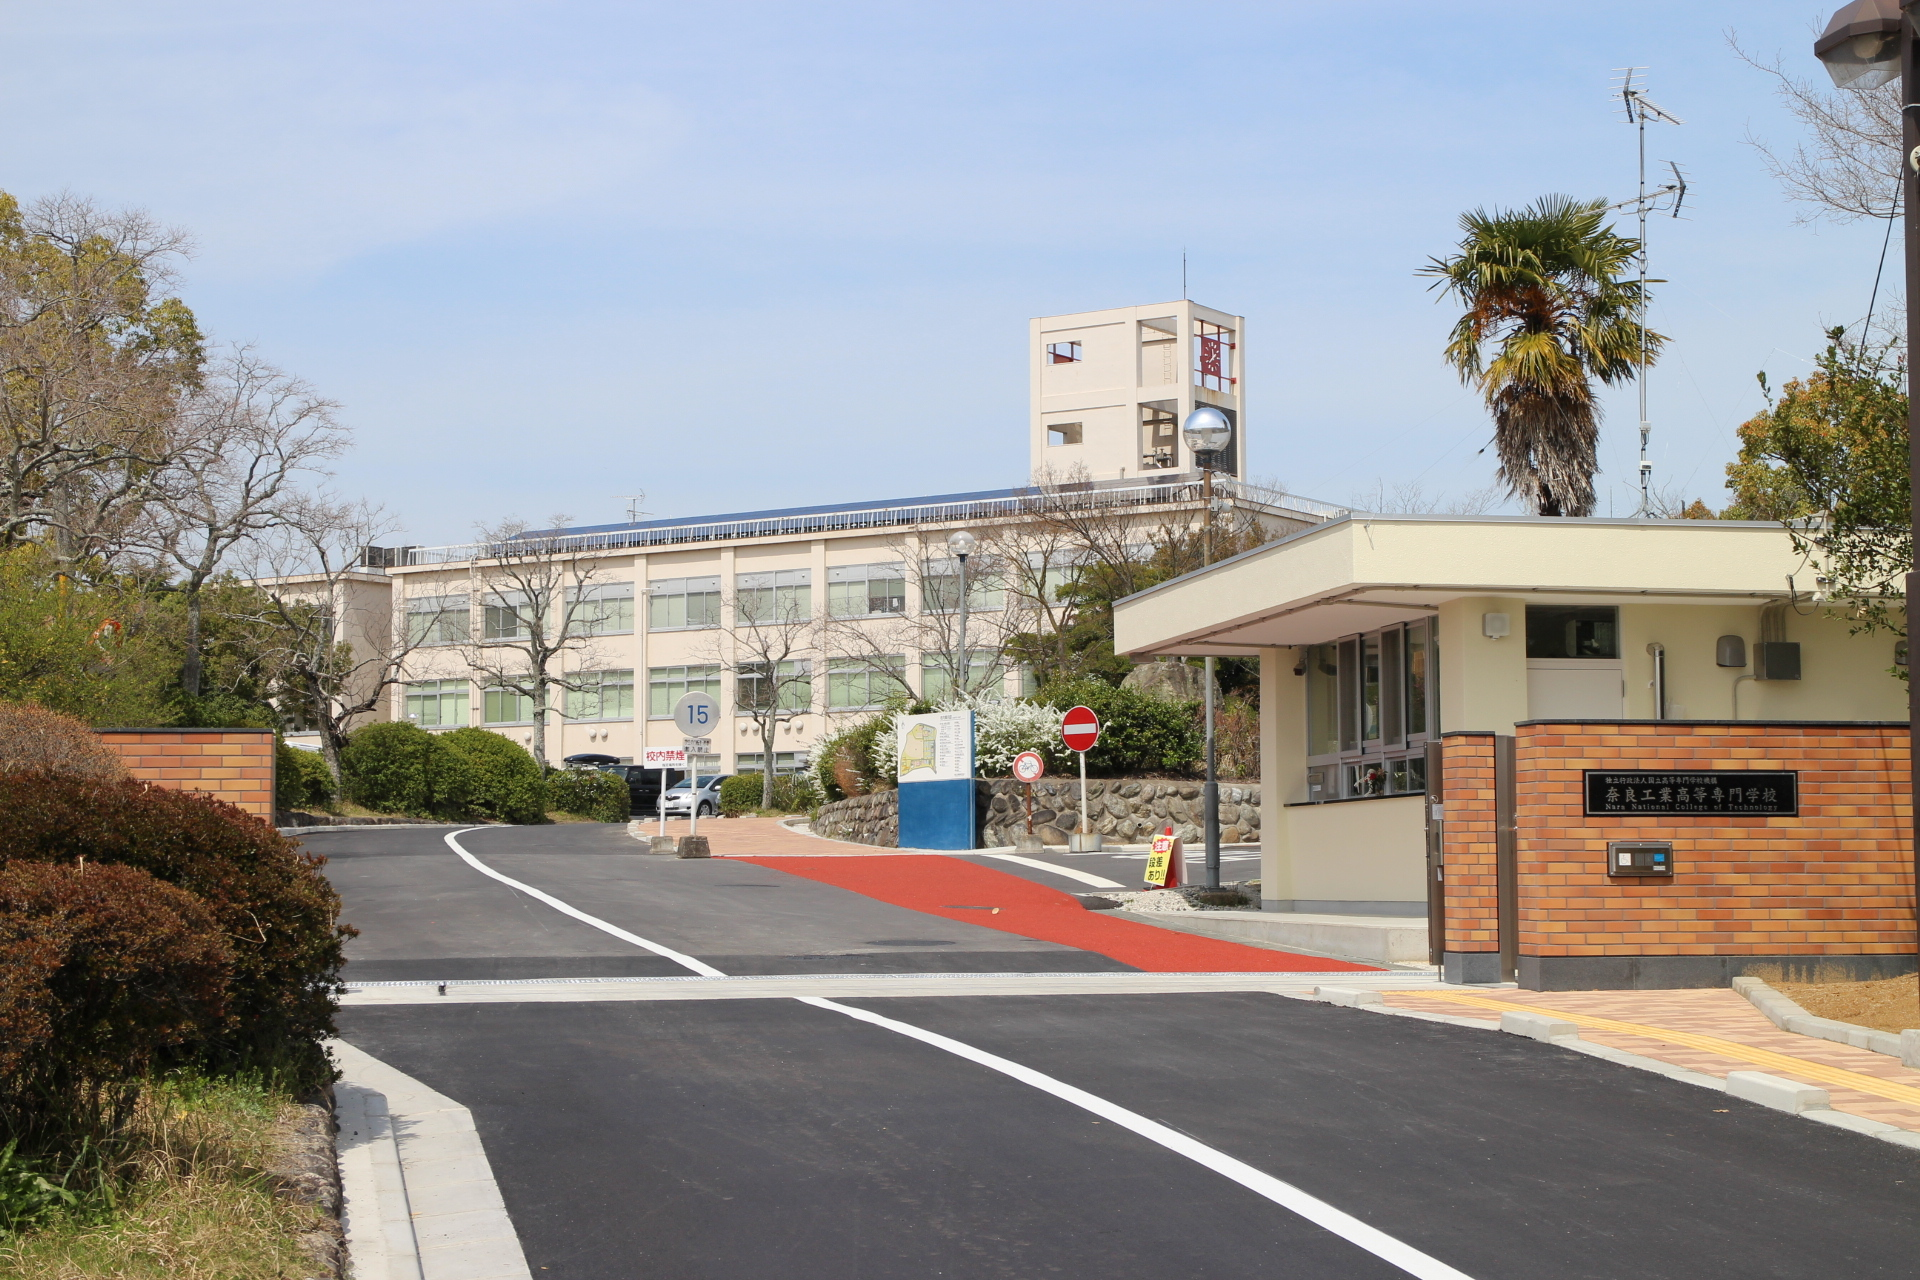
\includegraphics[width=5cm]{pic/nitnc.jpg}
    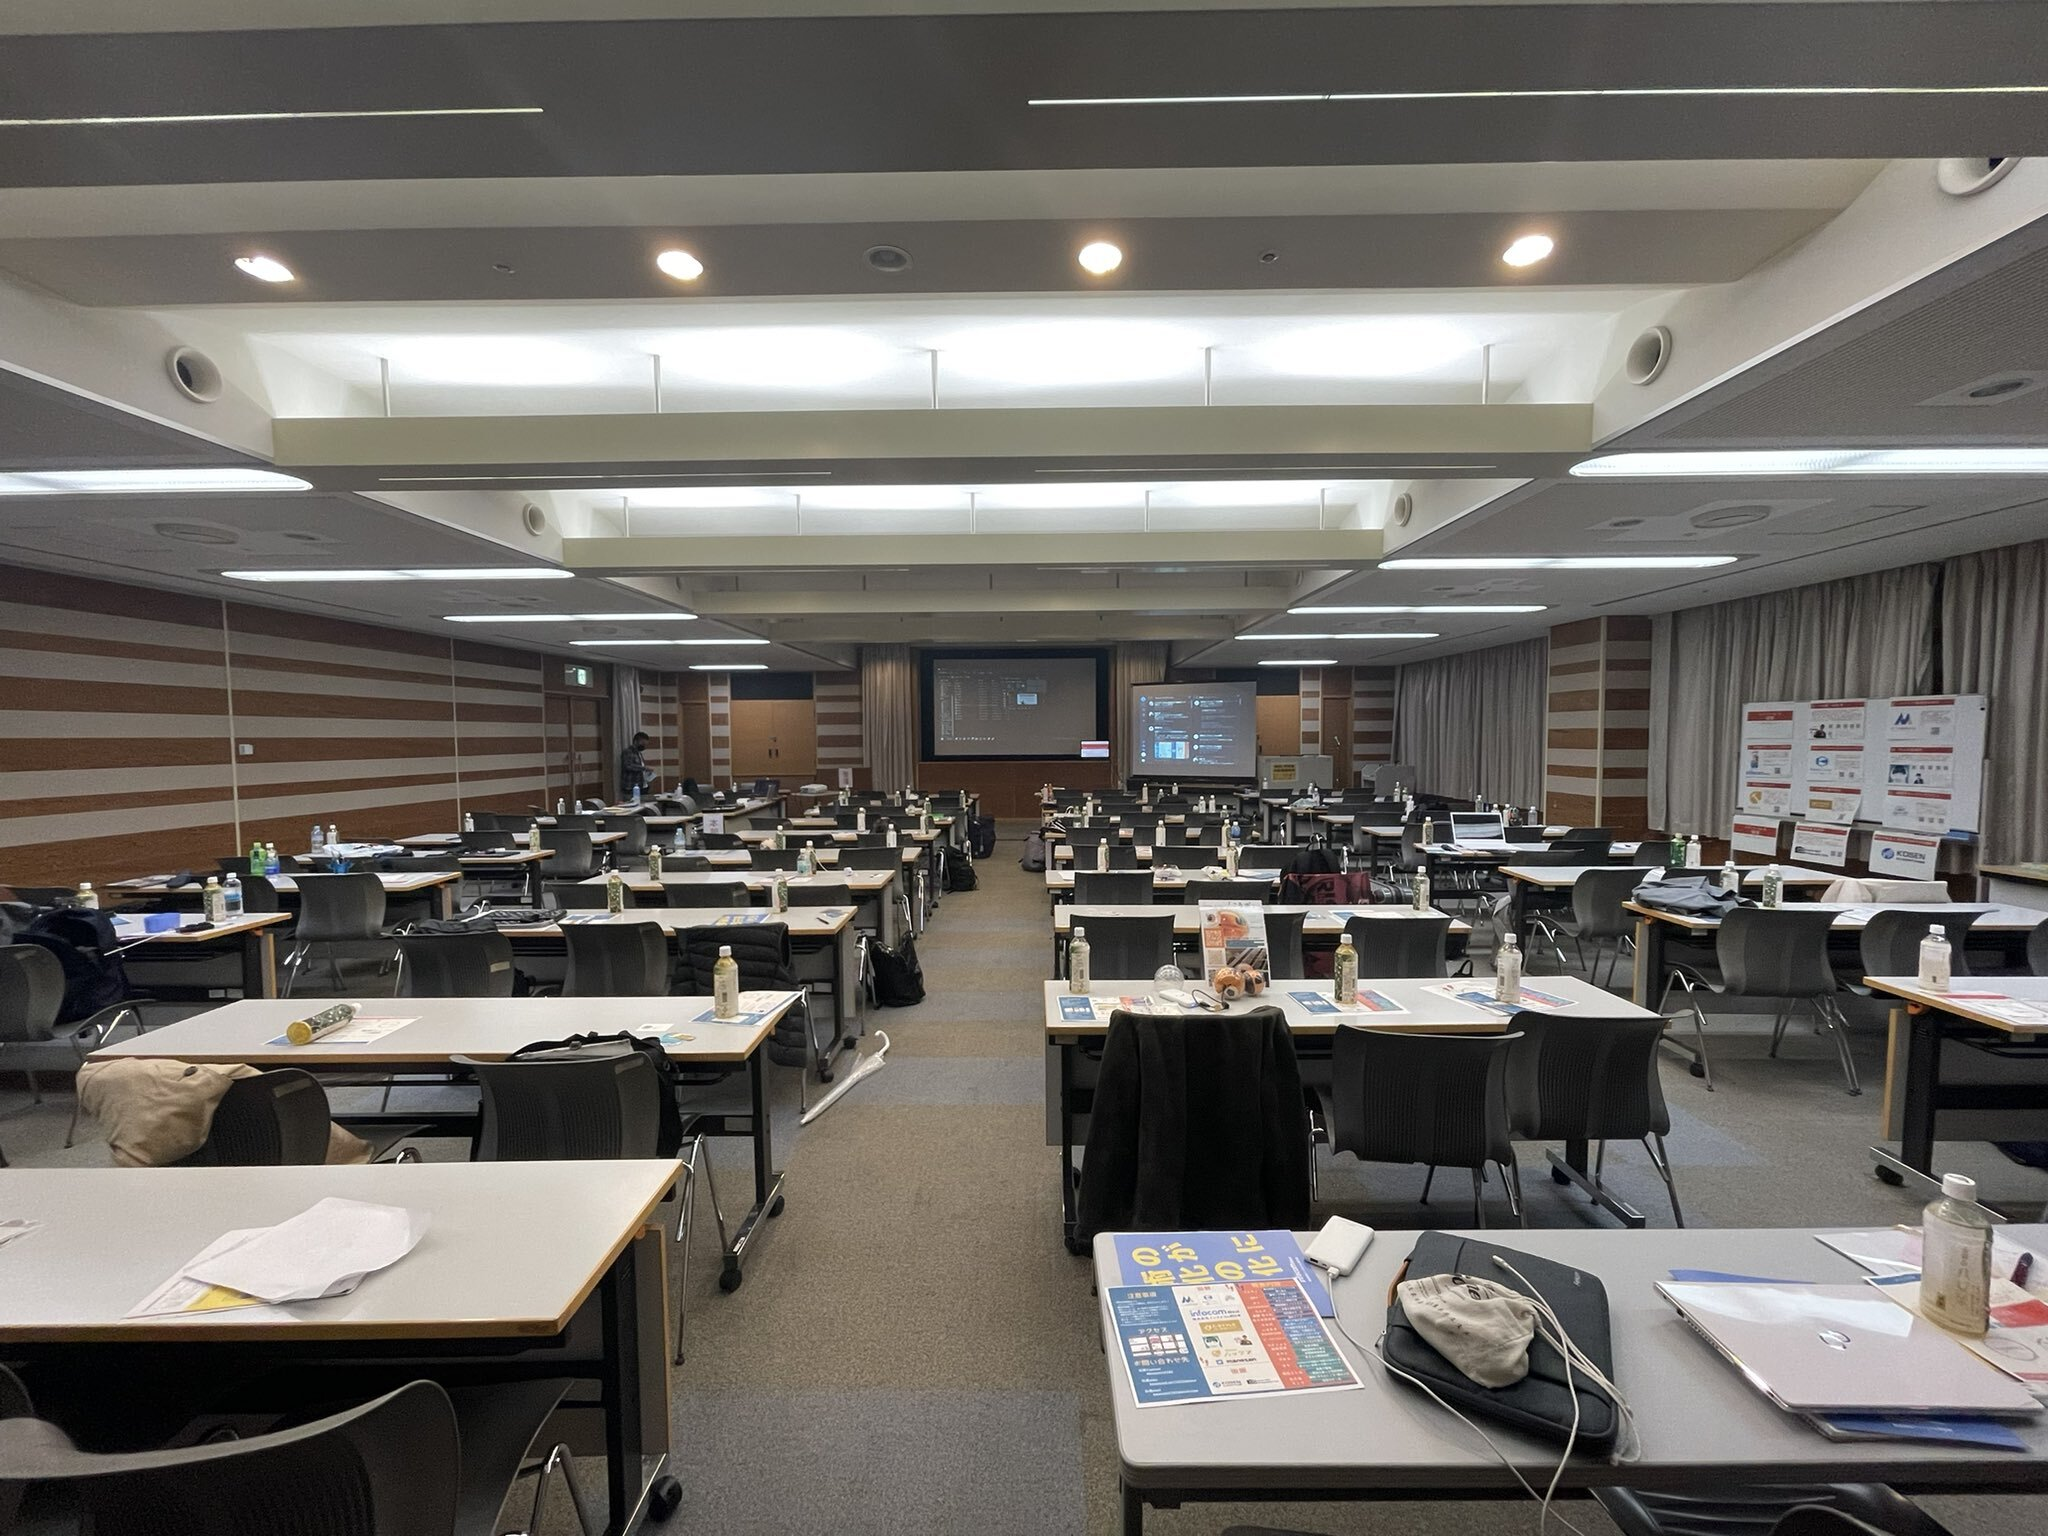
\includegraphics[width=5cm]{pic/Conf.jpg}
  \end{center}

\end{frame}

\begin{frame}{高専スタートアップ事業について}{時代は大高専時代に...}

  \begin{alertblock}{高専スタートアップ事業の3STEP}
    \begin{enumerate}
      \setlength{\itemsep}{1mm}
      \item アントレプレナーシップや起業について知る
      \item 高専生のチャレンジを応援するための環境整備\\
      $\Rightarrow$\alert{起業家工房}の整備
      \item 地域社会の課題解決に挑戦
    \end{enumerate}
  \end{alertblock}

  \begin{center}
    \begin{tikzpicture}[scale=.8]
      \node at (0,0) {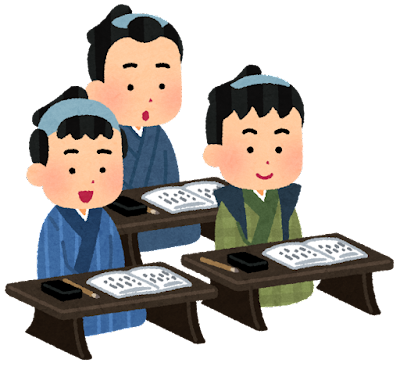
\includegraphics[width=3cm]{pic/learn.png}};
      \node at (5,0) {
\includegraphics[width=3cm]{pic/try.png}};
      \node at (10,0) {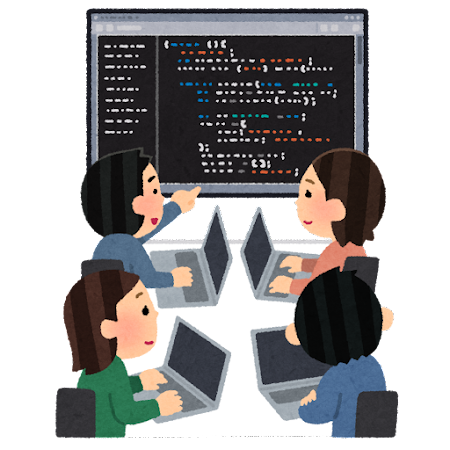
\includegraphics[width=3cm]{pic/team2.png}};
      \draw[-{Latex[length=5mm]},line width = 3pt] (2,0) -- (3,0);
      \draw[-{Latex[length=5mm]},line width = 3pt] (7,0) -- (8,0);
    \end{tikzpicture}
  \end{center}

\end{frame}

\begin{frame}{TechRingとは?}

  \begin{description}[一つの輪に]
    \item[学科の壁] 各学科には様々な長所や短所が混在するが...\par
    各学科が壁で隔てられ、\\長所を活かすことも短所を補うこともできない!\par
    \hspace{0.3\textwidth}
    
\begin{tikzpicture}
      \draw[-{Latex[length=5mm]},line width = 3pt,red] (0,.7) -- (0,0);
    \end{tikzpicture}
    \vspace{-1.5mm}
    \item[一つの輪に] 学科を超えた相互補完型の交流で\\\structure{究極のアントレプレナーシップ}を目指す!
  \end{description}

  \begin{columns}
    \begin{column}{0.55\textwidth}
      \begin{center}
        \begin{block}{TechRing 3つの起業}
          \vspace{2mm}
          \begin{enumerate}
            \setlength{\itemsep}{3mm}
            \item 学科交流イベントの起業
            \item 技術交流プロジェクトの起業
            \item 共同開発プロジェクトの起業
          \end{enumerate}
        \end{block}
      \end{center}
    \end{column}

    \begin{column}{0.40\textwidth}
      \begin{center}
        \begin{tikzpicture}[scale=1.4]
          %座標設定
          \coordinate (A) at (0,-.1);
          \coordinate (B) at (0,1);
          \coordinate (C) at ({cos(9*pi/10 r)},{sin(9*pi/10 r)});
          \coordinate (D) at ({cos(13*pi/10 r)},{sin(13*pi/10 r)});
          \coordinate (E) at ({cos(17*pi/10 r)},{sin(17*pi/10 r)});
          \coordinate (F) at ({cos(21*pi/10 r)},{sin(21*pi/10 r)});
          %線引き
          \draw[line width = 2pt] (F)--(B)--(C)--(D)--(E)--cycle;
          %nodeのスタイル指定
          \tikzset{block/.style={circle,white,fill=cyan,minimum size=1cm,inner sep=.5pt}};
          %node(テキストボックス的な)を指定座標に配置
          \node[inner sep=0pt] at (A) {\includegraphics[width=1.5cm]{pic/Logo.png}};
          \node[block] at (B) {\footnotesize MeCafe};
          \node[block] at (C) {\footnotesize メカ研};
          \node[block] at (D) {\footnotesize 電研};
          \node[block] at (E) {\footnotesize シス研};
          \node[block] at (F) {\footnotesize 情研};
        \end{tikzpicture}
      \end{center}
    \end{column}
  \end{columns}

\end{frame}

\begin{frame}{TechRing 3つの目的 その1}

  \begin{columns}[totalwidth=\textwidth]
    \begin{column}{0.7\textwidth}
      \begin{greyblock}{学科を超えた技術交流とその起業のために}
        \vspace{1mm}
        \begin{itemize}
          \item \alert{学内技術イベントを計画・運営}
          \item \alert{学内ロボットコンテストの共同開催}
          \item \alert{高専祭学科展にて相互連携}
        \end{itemize}
      \end{greyblock}
    \end{column}
    \begin{column}{0.25\textwidth}
      
\includegraphics[scale=.25]{pic/mokuhyou1.png}
    \end{column}
  \end{columns}

  \begin{columns}
    \begin{column}{0.30\textwidth}
      \begin{alertblock}{学内イベント}
        \begin{footnotesize}
          TechRing 3つの起業
          \begin{enumerate}
            \item 学科交流\\Eventの起業
          \end{enumerate}
        \end{footnotesize}
      \end{alertblock}
    \end{column}

    \begin{column}{0.30\textwidth}
      \begin{block}{技術交流}
        \begin{footnotesize}
          TechRing 3つの起業
          \begin{enumerate}
            \setcounter{enumi}{1}
            \item 技術交流\\Projectの起業
          \end{enumerate}
        \end{footnotesize}
      \end{block}
    \end{column}

    \begin{column}{0.30\textwidth}
      \begin{block}{共同制作}
        \begin{footnotesize}
          TechRing 3つの起業 \par
          \begin{enumerate}
            \setcounter{enumi}{2}
            \item 共同開発\\Projectの起業
          \end{enumerate}
        \end{footnotesize}
      \end{block}
    \end{column}
  \end{columns}
\end{frame}

\begin{frame}{TechRing 3つの活動 その1}{イベント運営}
  \begin{columns}[totalwidth=\textwidth]
    \begin{column}{0.55\textwidth}
      \begin{alertblock}{TechCafe}
        \begin{itemize}
          \item 年に一度の学内一大\\LTイベントとして開催
          \item 技術発表に限らない\\幅広いテーマ設定
          \item 高専祭のアフターイベント\\としてバックアップ
        \end{itemize}
      \end{alertblock}

      \begin{block}{他にも}
        \begin{footnotesize}
          \begin{itemize}
            \item 高専祭学科展にて連携
            \item \alert{TEDxNaraKOSEN}やりたい!
            \item 学内ロボコンできたらいいな
          \end{itemize}
        \end{footnotesize}
      \end{block}
    \end{column}

    \begin{column}{0.4\textwidth}
      \begin{greyblock}{TalkCafeの様子}
        \begin{center}
          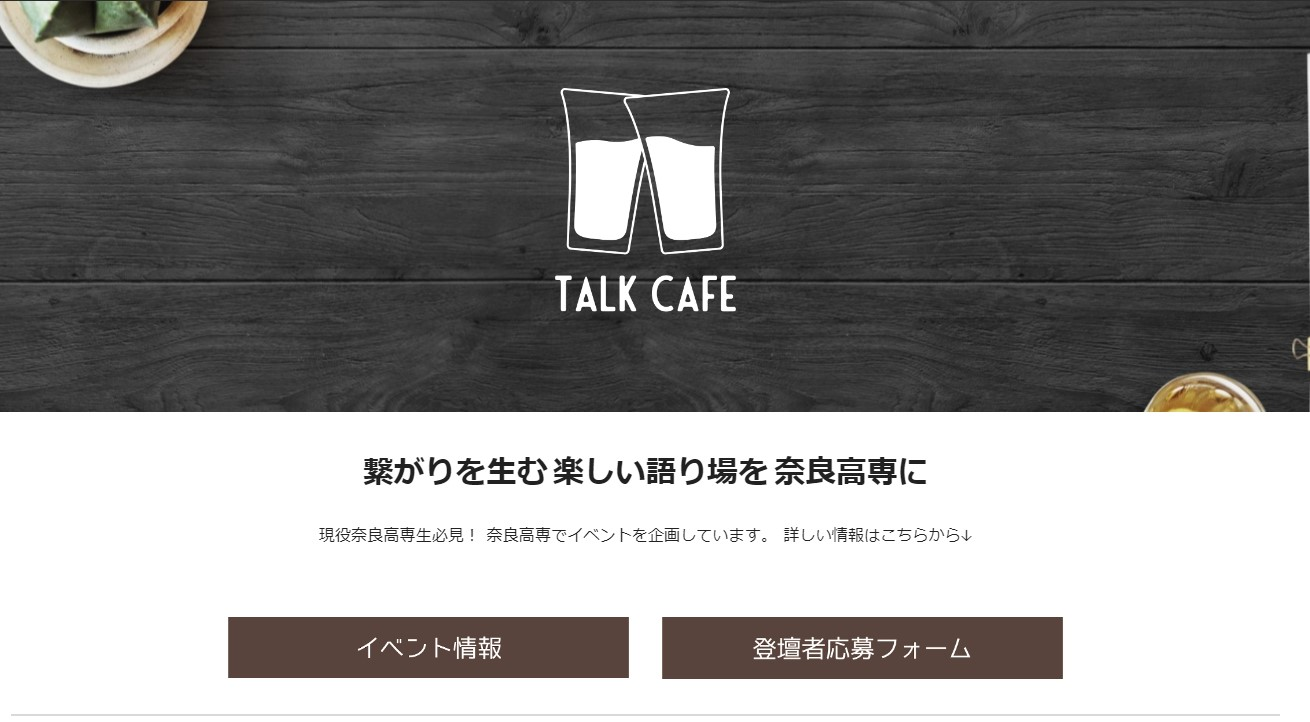
\includegraphics[scale=.12]{pic/TalkCafeHP.jpg}\\
          \vspace{2mm}
          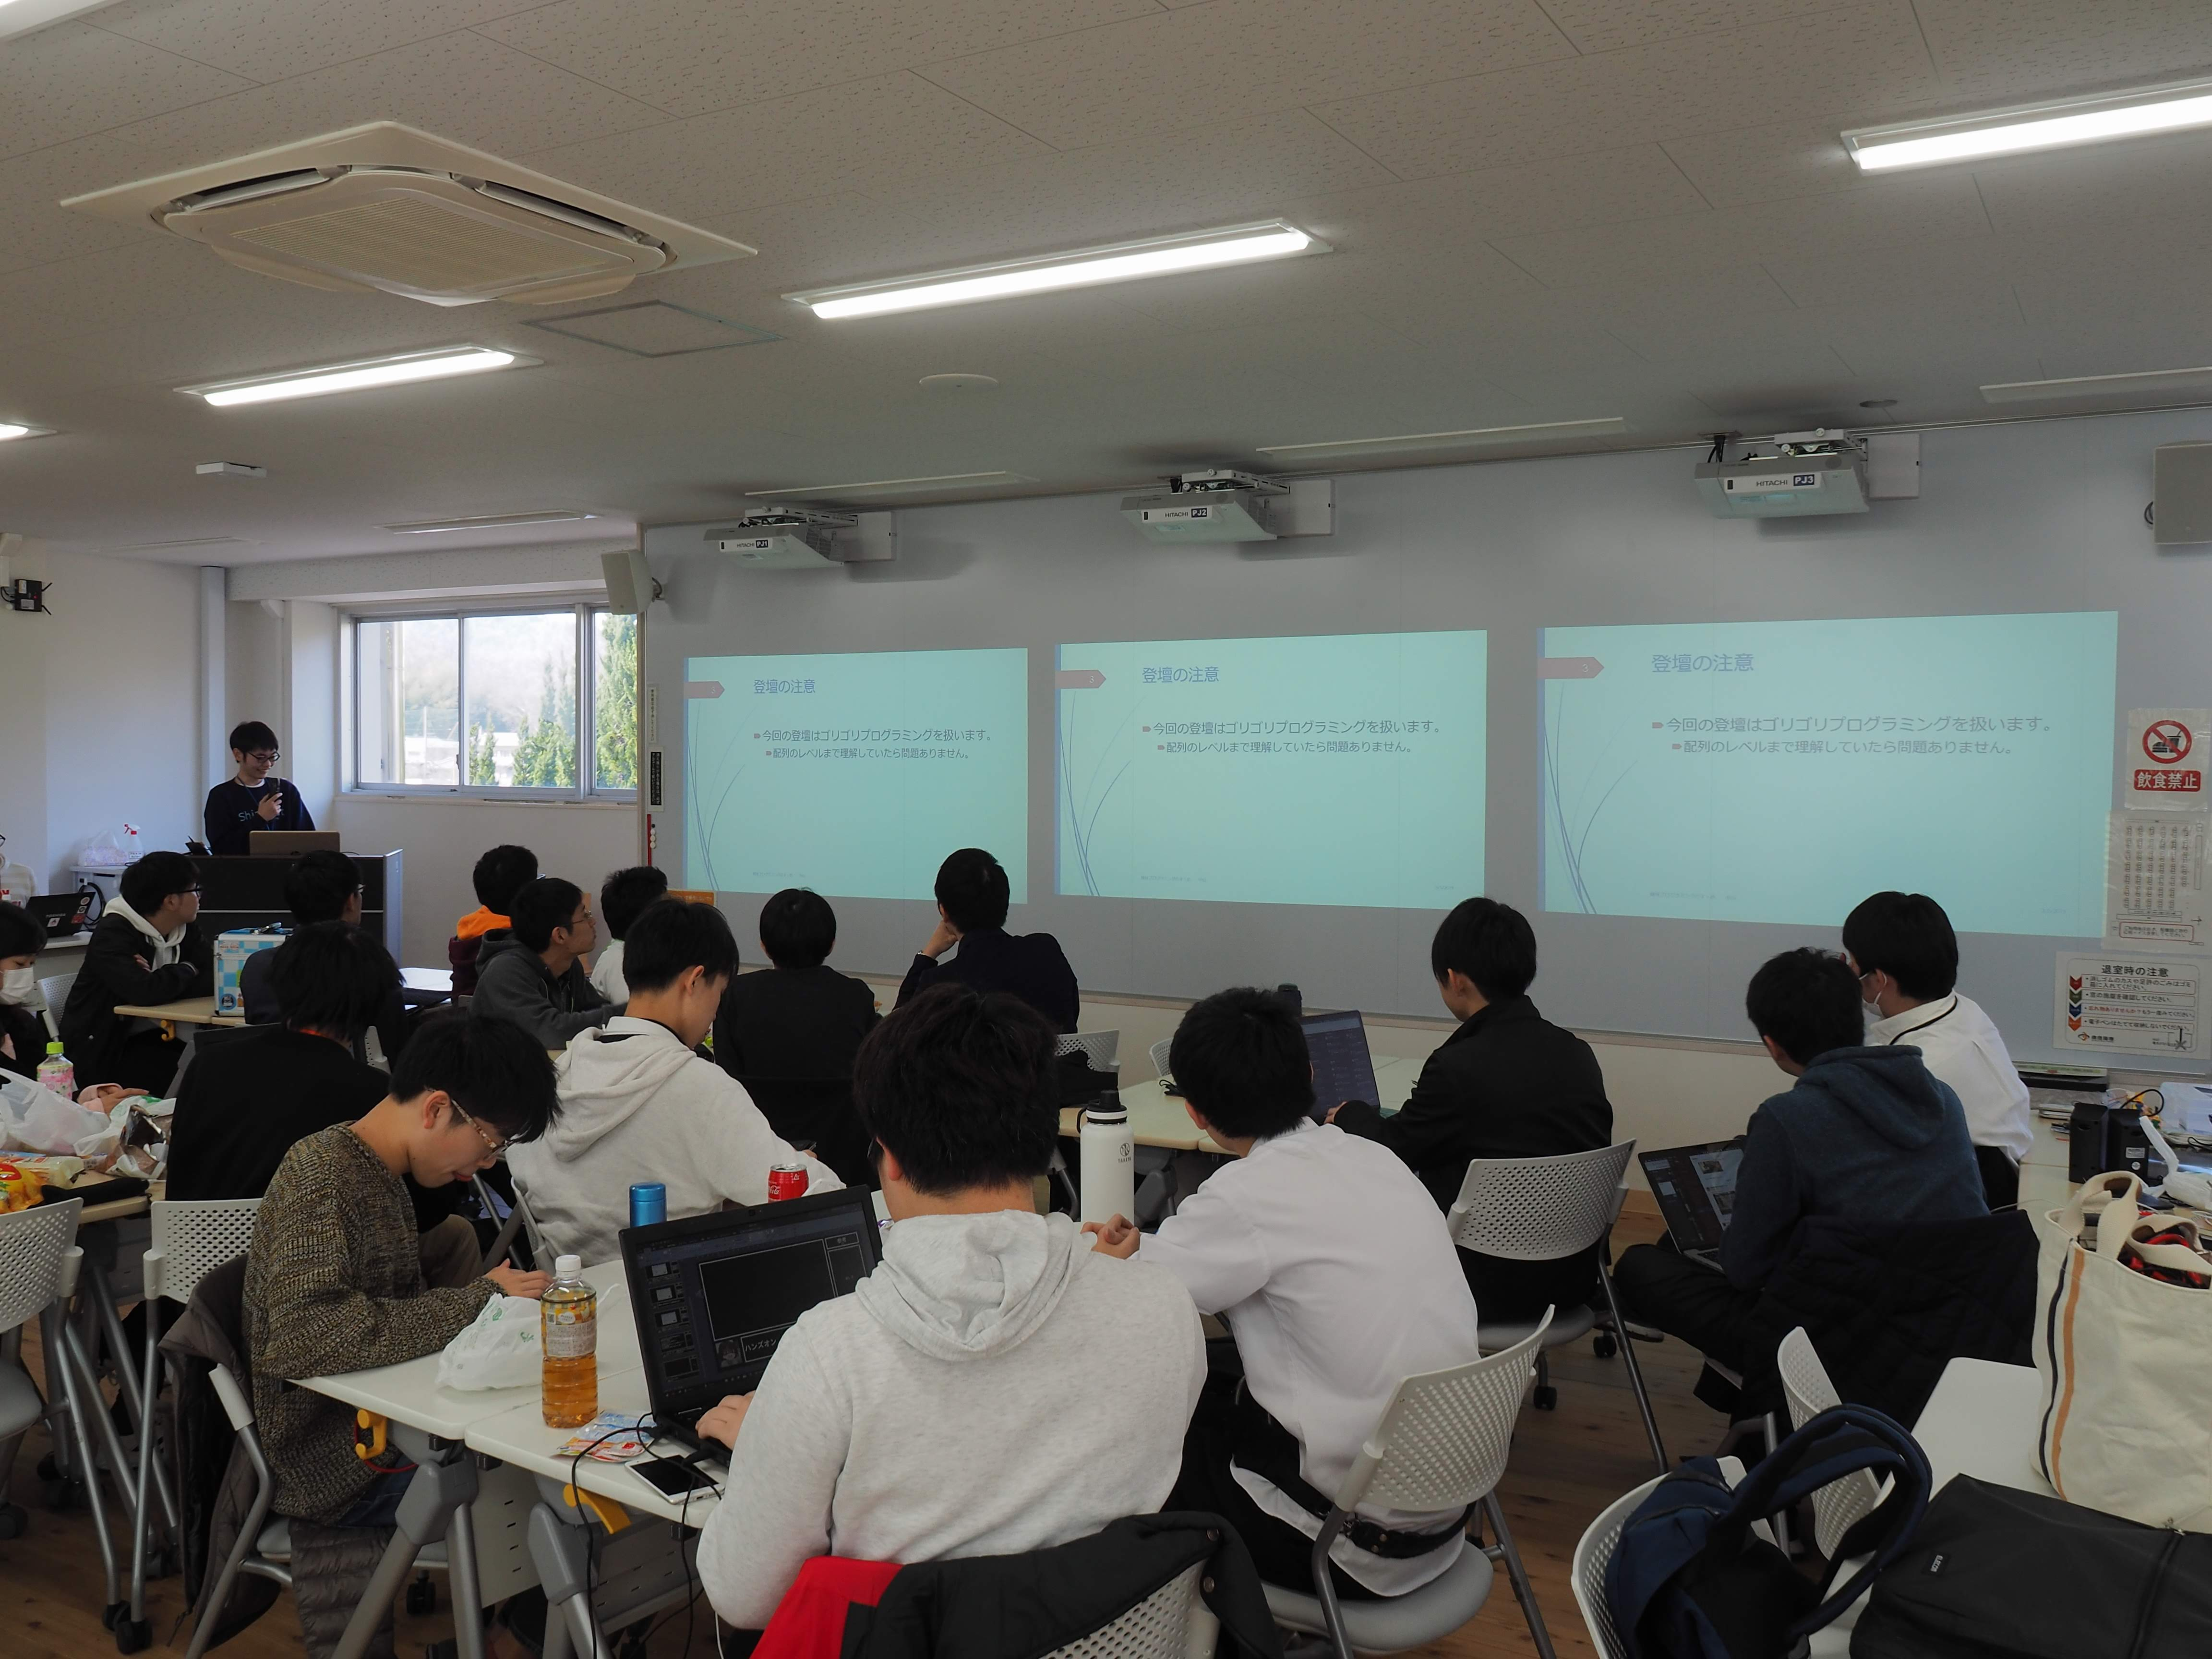
\includegraphics[scale=.025]{pic/TalkCafe.jpg}
        \end{center}
      \end{greyblock}
    \end{column}
  \end{columns}
\end{frame}

\begin{frame}{TechRing 3つの目的 その2}

  \begin{columns}[totalwidth=\textwidth]
    \begin{column}{0.7\textwidth}
      \begin{greyblock}{学科を超えた技術交流とその起業のために}
        \vspace{1mm}
        \begin{itemize}
          \item \alert{TechRing内技術交流}
          \item \alert{他高専の有志・団体との交流}
          \item \alert{各種コンテスト、展示会への出場}
        \end{itemize}
      \end{greyblock}
    \end{column}
    \begin{column}{0.25\textwidth}
      
\includegraphics[scale=.25]{pic/mokuhyou2.png}
    \end{column}
  \end{columns}

  \begin{columns}
    \begin{column}{0.30\textwidth}
      \begin{block}{学内イベント}
        \begin{footnotesize}
          TechRing 3つの起業
          \begin{enumerate}
            \item 学科交流\\Eventの起業
          \end{enumerate}
        \end{footnotesize}
      \end{block}
    \end{column}

    \begin{column}{0.30\textwidth}
      \begin{alertblock}{技術交流}
        \begin{footnotesize}
          TechRing 3つの起業
          \begin{enumerate}
            \setcounter{enumi}{1}
            \item 技術交流\\Projectの起業
          \end{enumerate}
        \end{footnotesize}
      \end{alertblock}
    \end{column}

    \begin{column}{0.30\textwidth}
      \begin{block}{共同制作}
        \begin{footnotesize}
          TechRing 3つの起業 \par
          \begin{enumerate}
            \setcounter{enumi}{2}
            \item 共同開発\\Projectの起業
          \end{enumerate}
        \end{footnotesize}
      \end{block}
    \end{column}
  \end{columns}
\end{frame}

\begin{frame}{TechRing 3つの活動 その2}{技術交流}

  \begin{columns}[totalwidth=\textwidth]
    \begin{column}{0.76\textwidth}
      \begin{alertblock}{TechRingミーティング}
        \begin{itemize}
          \item 定期的な活動報告会
          \item 様々なノウハウの共有
        \end{itemize}
      \end{alertblock}
    
      \begin{alertblock}{Maker Faire Kyoto 2023 出展}
          \begin{itemize}
            \item 各団体が製作した製作品のアウトプット
            \item 共同展示の連携で、TechRing認知度の向上
          \end{itemize}
      \end{alertblock}
    \end{column}

    \begin{column}{0.2\textwidth}
      \begin{center}
        
\includegraphics[scale=.18]{pic/discuss.png}
      \end{center}
    \end{column}
  \end{columns}

  \begin{block}{製作品外部公開}
    \begin{itemize}
      \item 奈良高専外部との交流も深める
      \item 外部の意見も取り入れ、より良い展示品に
    \end{itemize}
  \end{block}
\end{frame}

\begin{frame}{TechRing 3つの目的 その3}

  \begin{columns}[totalwidth=\textwidth]
    \begin{column}{0.7\textwidth}
      \begin{greyblock}{学科を超えた技術交流とその起業のために}
        \vspace{1mm}
        \begin{itemize}
          \item \alert{各種コンテスト、展示会への出場}
          \item \alert{共同開発プロジェクトの企画}
          \item \alert{チャレンジプロジェクトに参加}
        \end{itemize}
        \end{greyblock}
    \end{column}
    \begin{column}{0.25\textwidth}
      
\includegraphics[scale=.25]{pic/mokuhyou3.png}
    \end{column}
  \end{columns}

  \begin{columns}
    \begin{column}{0.30\textwidth}
      \begin{block}{学内イベント}
        \begin{footnotesize}
          TechRing 3つの起業
          \begin{enumerate}
            \item 学科交流\\Eventの起業
          \end{enumerate}
        \end{footnotesize}
      \end{block}
    \end{column}

    \begin{column}{0.30\textwidth}
      \begin{block}{技術交流}
        \begin{footnotesize}
          TechRing 3つの起業
          \begin{enumerate}
            \setcounter{enumi}{1}
            \item 技術交流\\Projectの起業
          \end{enumerate}
        \end{footnotesize}
      \end{block}
    \end{column}

    \begin{column}{0.30\textwidth}
      \begin{alertblock}{共同制作}
        \begin{footnotesize}
          TechRing 3つの起業 \par
          \begin{enumerate}
            \setcounter{enumi}{2}
            \item 共同開発\\Projectの起業
          \end{enumerate}
        \end{footnotesize}
      \end{alertblock}
    \end{column}
  \end{columns}
\end{frame}

\begin{frame}{TechRing 3つの活動 その3}{共同開発}
  \begin{columns}
    \begin{column}{0.63\textwidth}
      \begin{block}{開発環境の整備}
        \begin{itemize}
          \item 起業家工房の環境を整備
          \item 起業家工房による\\有志個人のものづくり支援も
        \end{itemize}
      \end{block}
    \end{column}

    \begin{column}{0.28\textwidth}
      \begin{center}
        
\includegraphics[width=2.5cm]{pic/Team.png}
      \end{center}
    \end{column}
  \end{columns}

  \begin{alertblock}{共同開発プロジェクト}
    \begin{itemize}
      \item 学科を跨いだ人員を確保し、コンテスト共同参加
      \item 学校の枠組みを超えた、様々なサービス共同開発
      \item 開発したサービスを、地域社会に提供
    \end{itemize}
  \end{alertblock}
\end{frame}

\begin{frame}{TechRingの組成}{3つの起業を5つの団体で}
  \begin{tikzpicture}[overlay]
    \node at (9, 1.2){
\includegraphics[scale=.15]{pic/team3.png}};
    \node at (9, -3.8){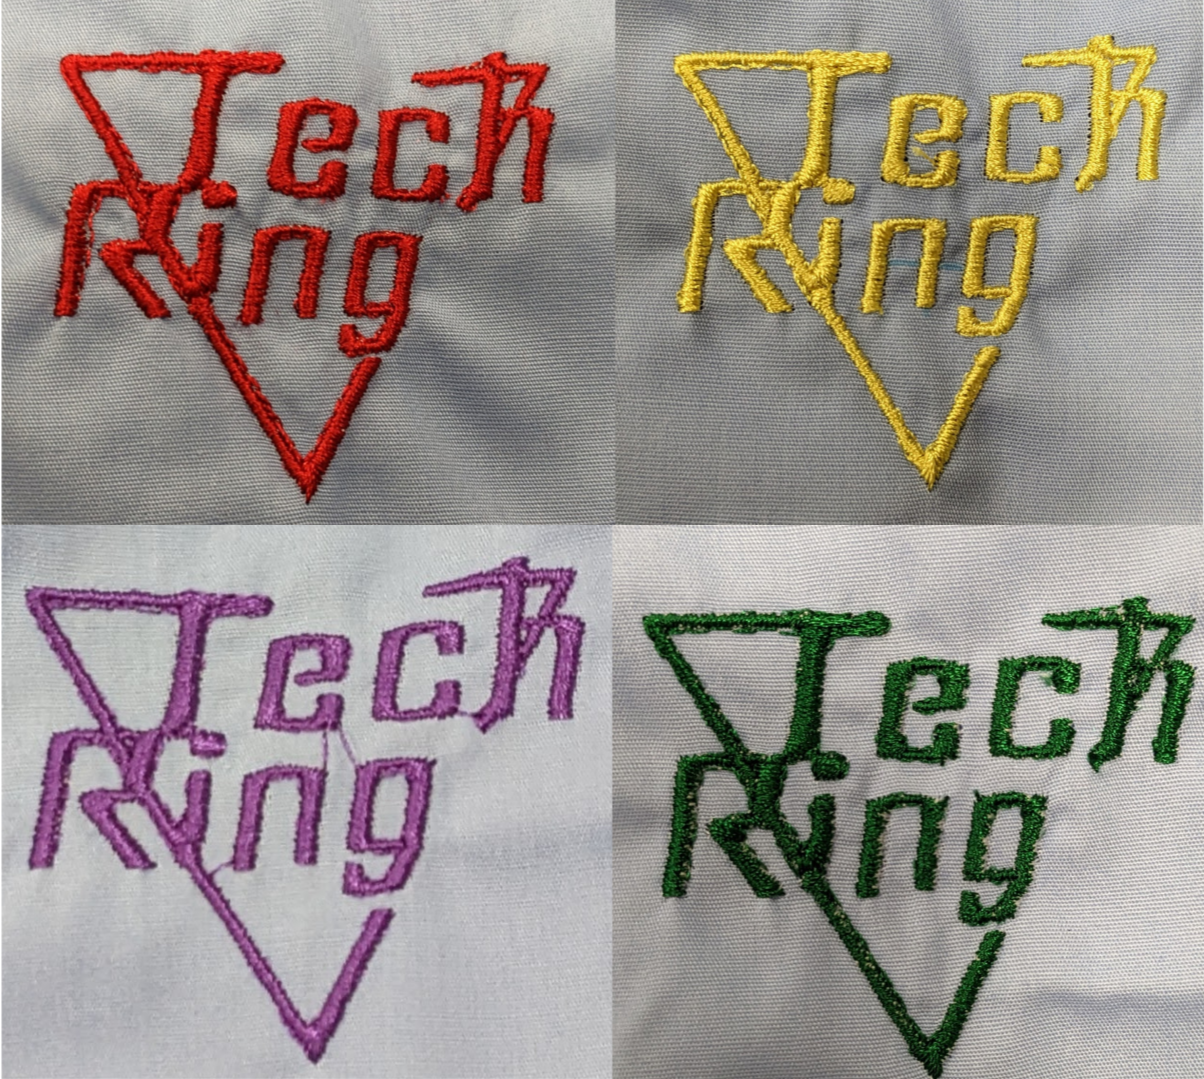
\includegraphics[scale=.08]{pic/TechRing.png}};
  \end{tikzpicture}

  \vspace{-5mm}

  \begin{block}{何処から誰を招集するか}
    \vspace{2mm}
    \begin{description}
      \setlength{\itemsep}{2mm}
      \item[招集基準] 各学科を代表する団体を招集したい
      \item[判断素材] 高専祭学科展の展示に携わった経験のある団体
      \item[招集結果] 4学科から5団体の参加が確定!
    \end{description}
  \end{block}

  \begin{center}
    
\begin{tikzpicture}
      \draw[-{Latex[length=5mm]},line width = 3pt,red] (0,.7) -- (0,0);
    \end{tikzpicture}
  \end{center}

  \begin{Large}
    各学科各団体の\alert{長所を活かし} \vfill \hspace{5em}\alert{短所を補う}プロジェクトとして発足!
  \end{Large}
\end{frame}

\begin{frame}{TechRingを創る仲間たち その1}{MeCafe}

  \vspace{-2mm}
  
  \begin{minipage}{0.85\textwidth}
    \begin{block}{活動内容}
      \begin{itemize}
        \item 自分の中の「アイディア」を「カタチ」に
        \item モノを使ったコトづくりを
      \end{itemize}
    \end{block}
  \end{minipage}

  \begin{columns}[totalwidth=1.02\textwidth]
    \begin{column}{.3\textwidth}
      \begin{footnotesize}
        \begin{alertblock}{\normalsize Generative Design}
            \begin{center}
              パラメータから\\
              AIが設計案を導出\\
            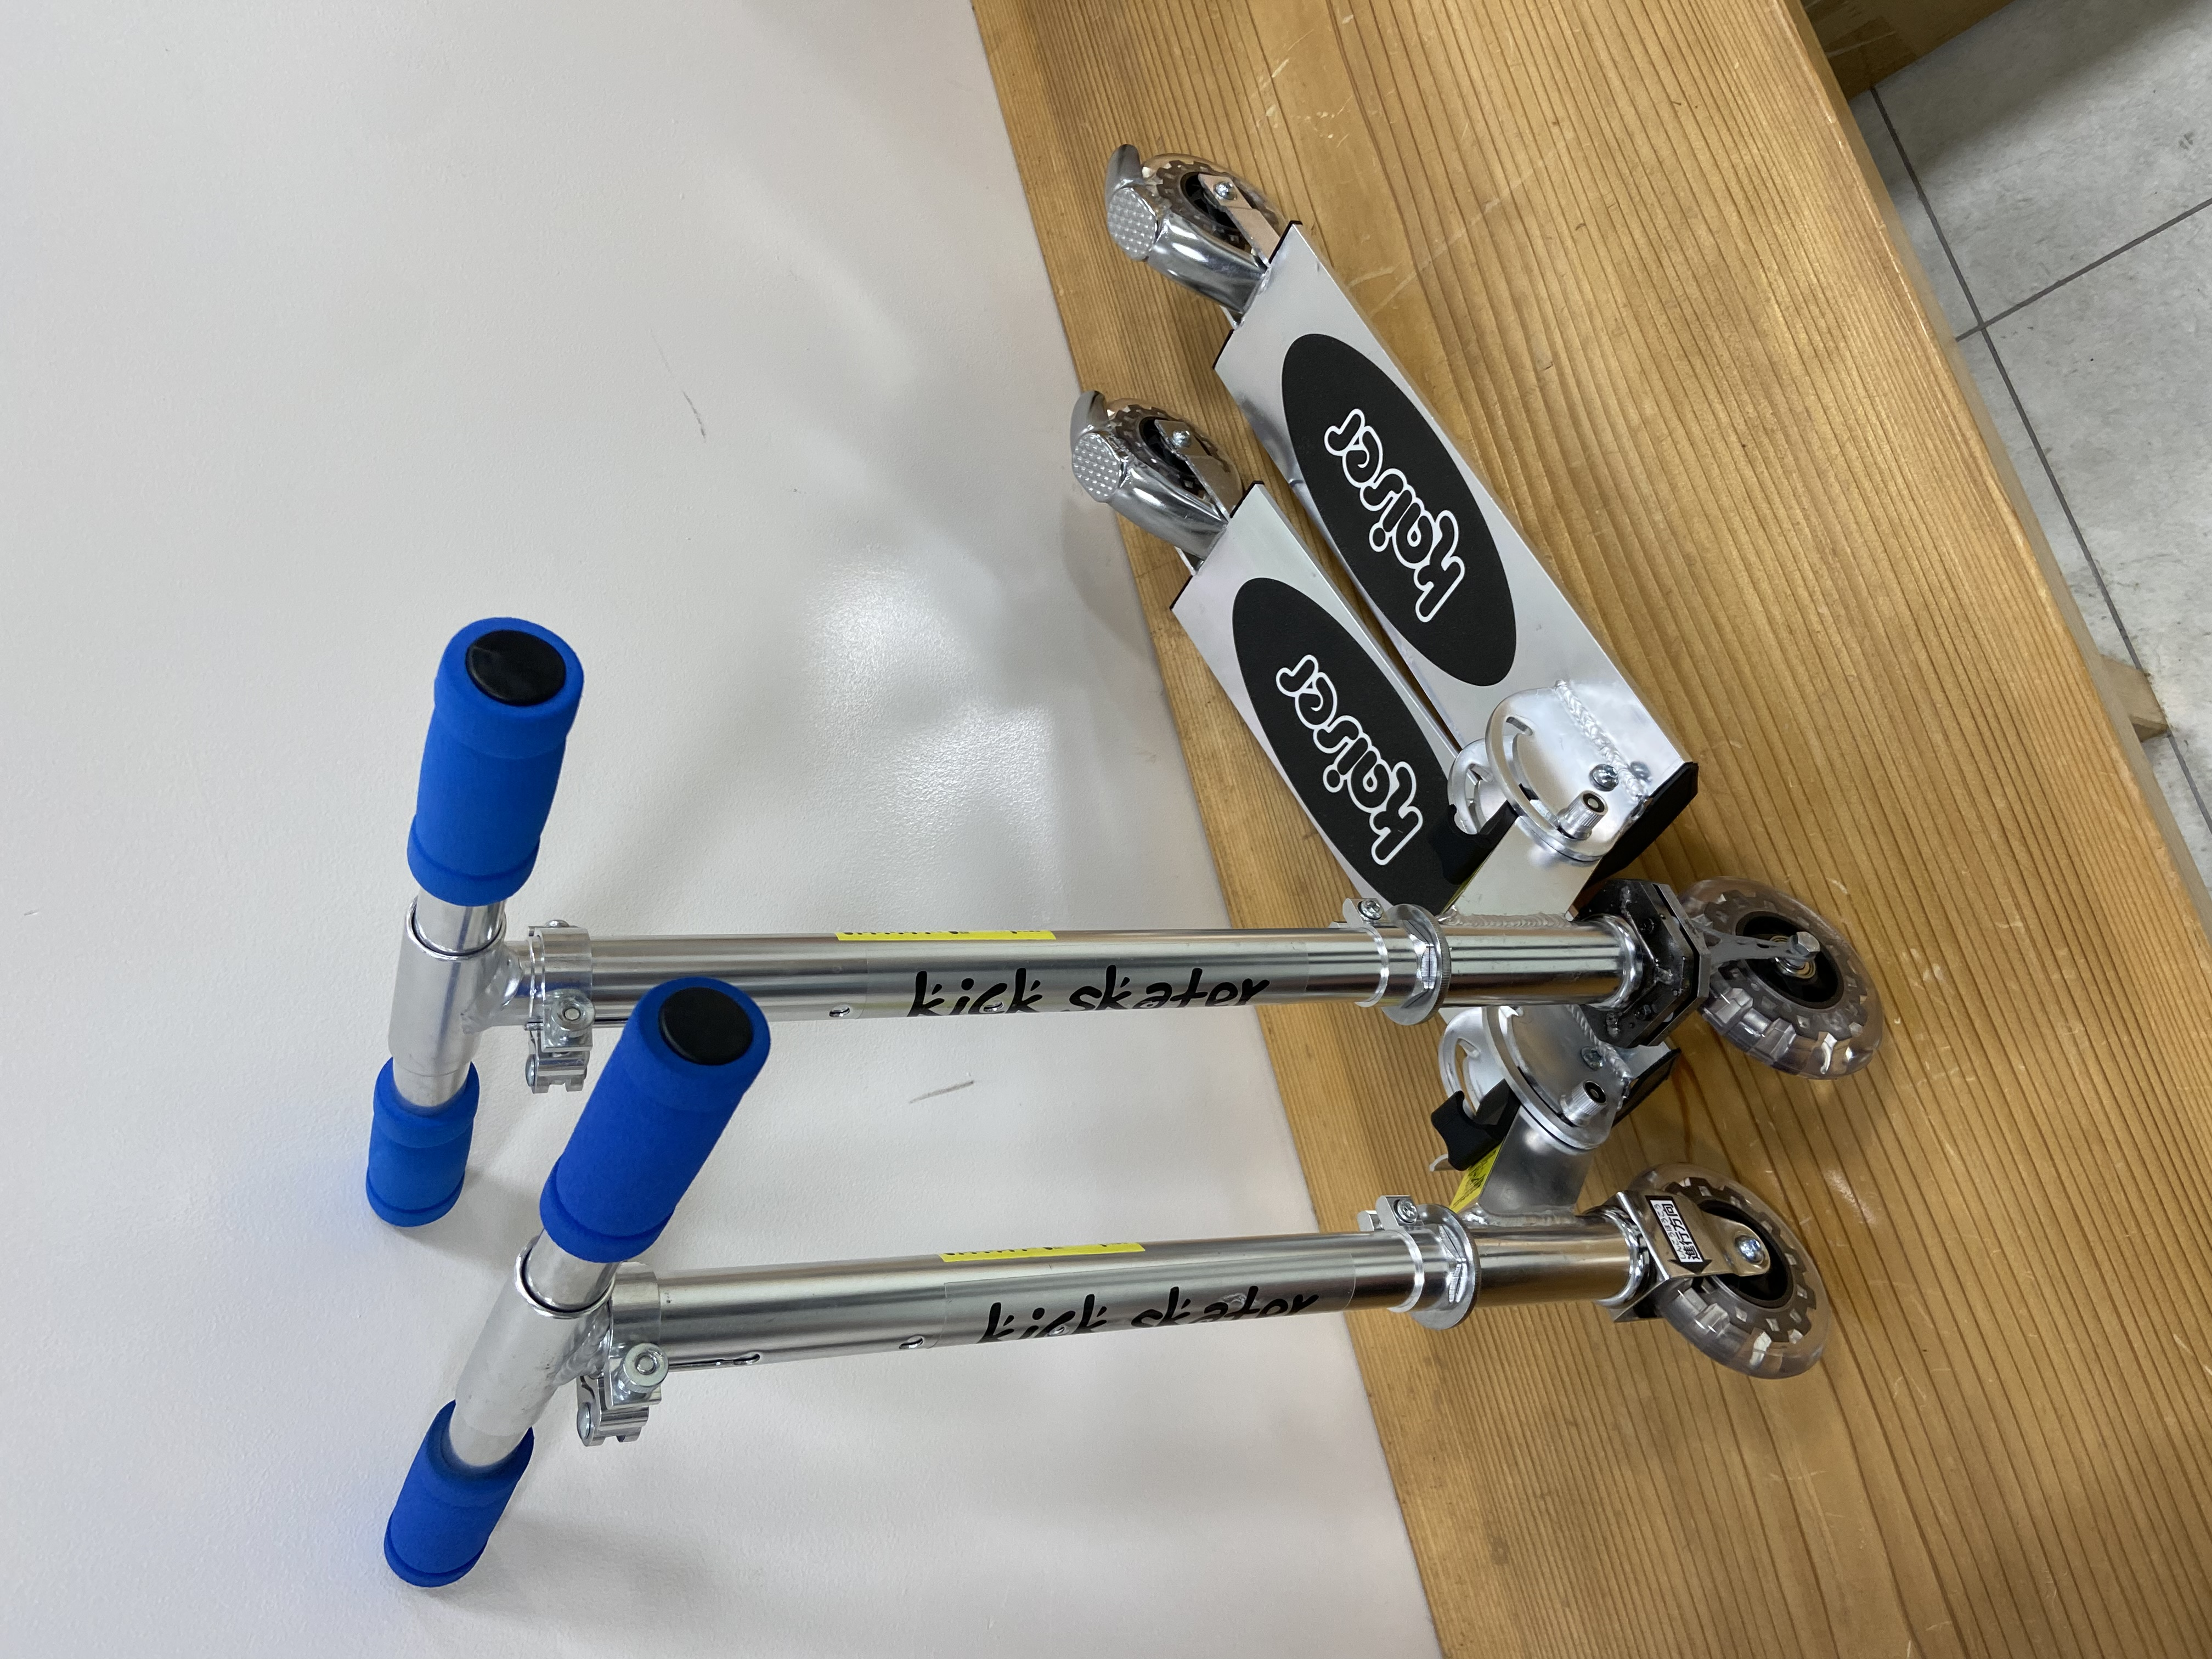
\includegraphics[scale=.02,angle=-90]{pic/mecafe1.jpg}
            \end{center}
        \end{alertblock}
      \end{footnotesize}
    \end{column}
    \begin{column}{.3\textwidth}
      \begin{footnotesize}
        \begin{alertblock}{テキサンラジコンカー}
          \begin{center}
            MGを加工して\\
            ラジコンカーを製作\\
            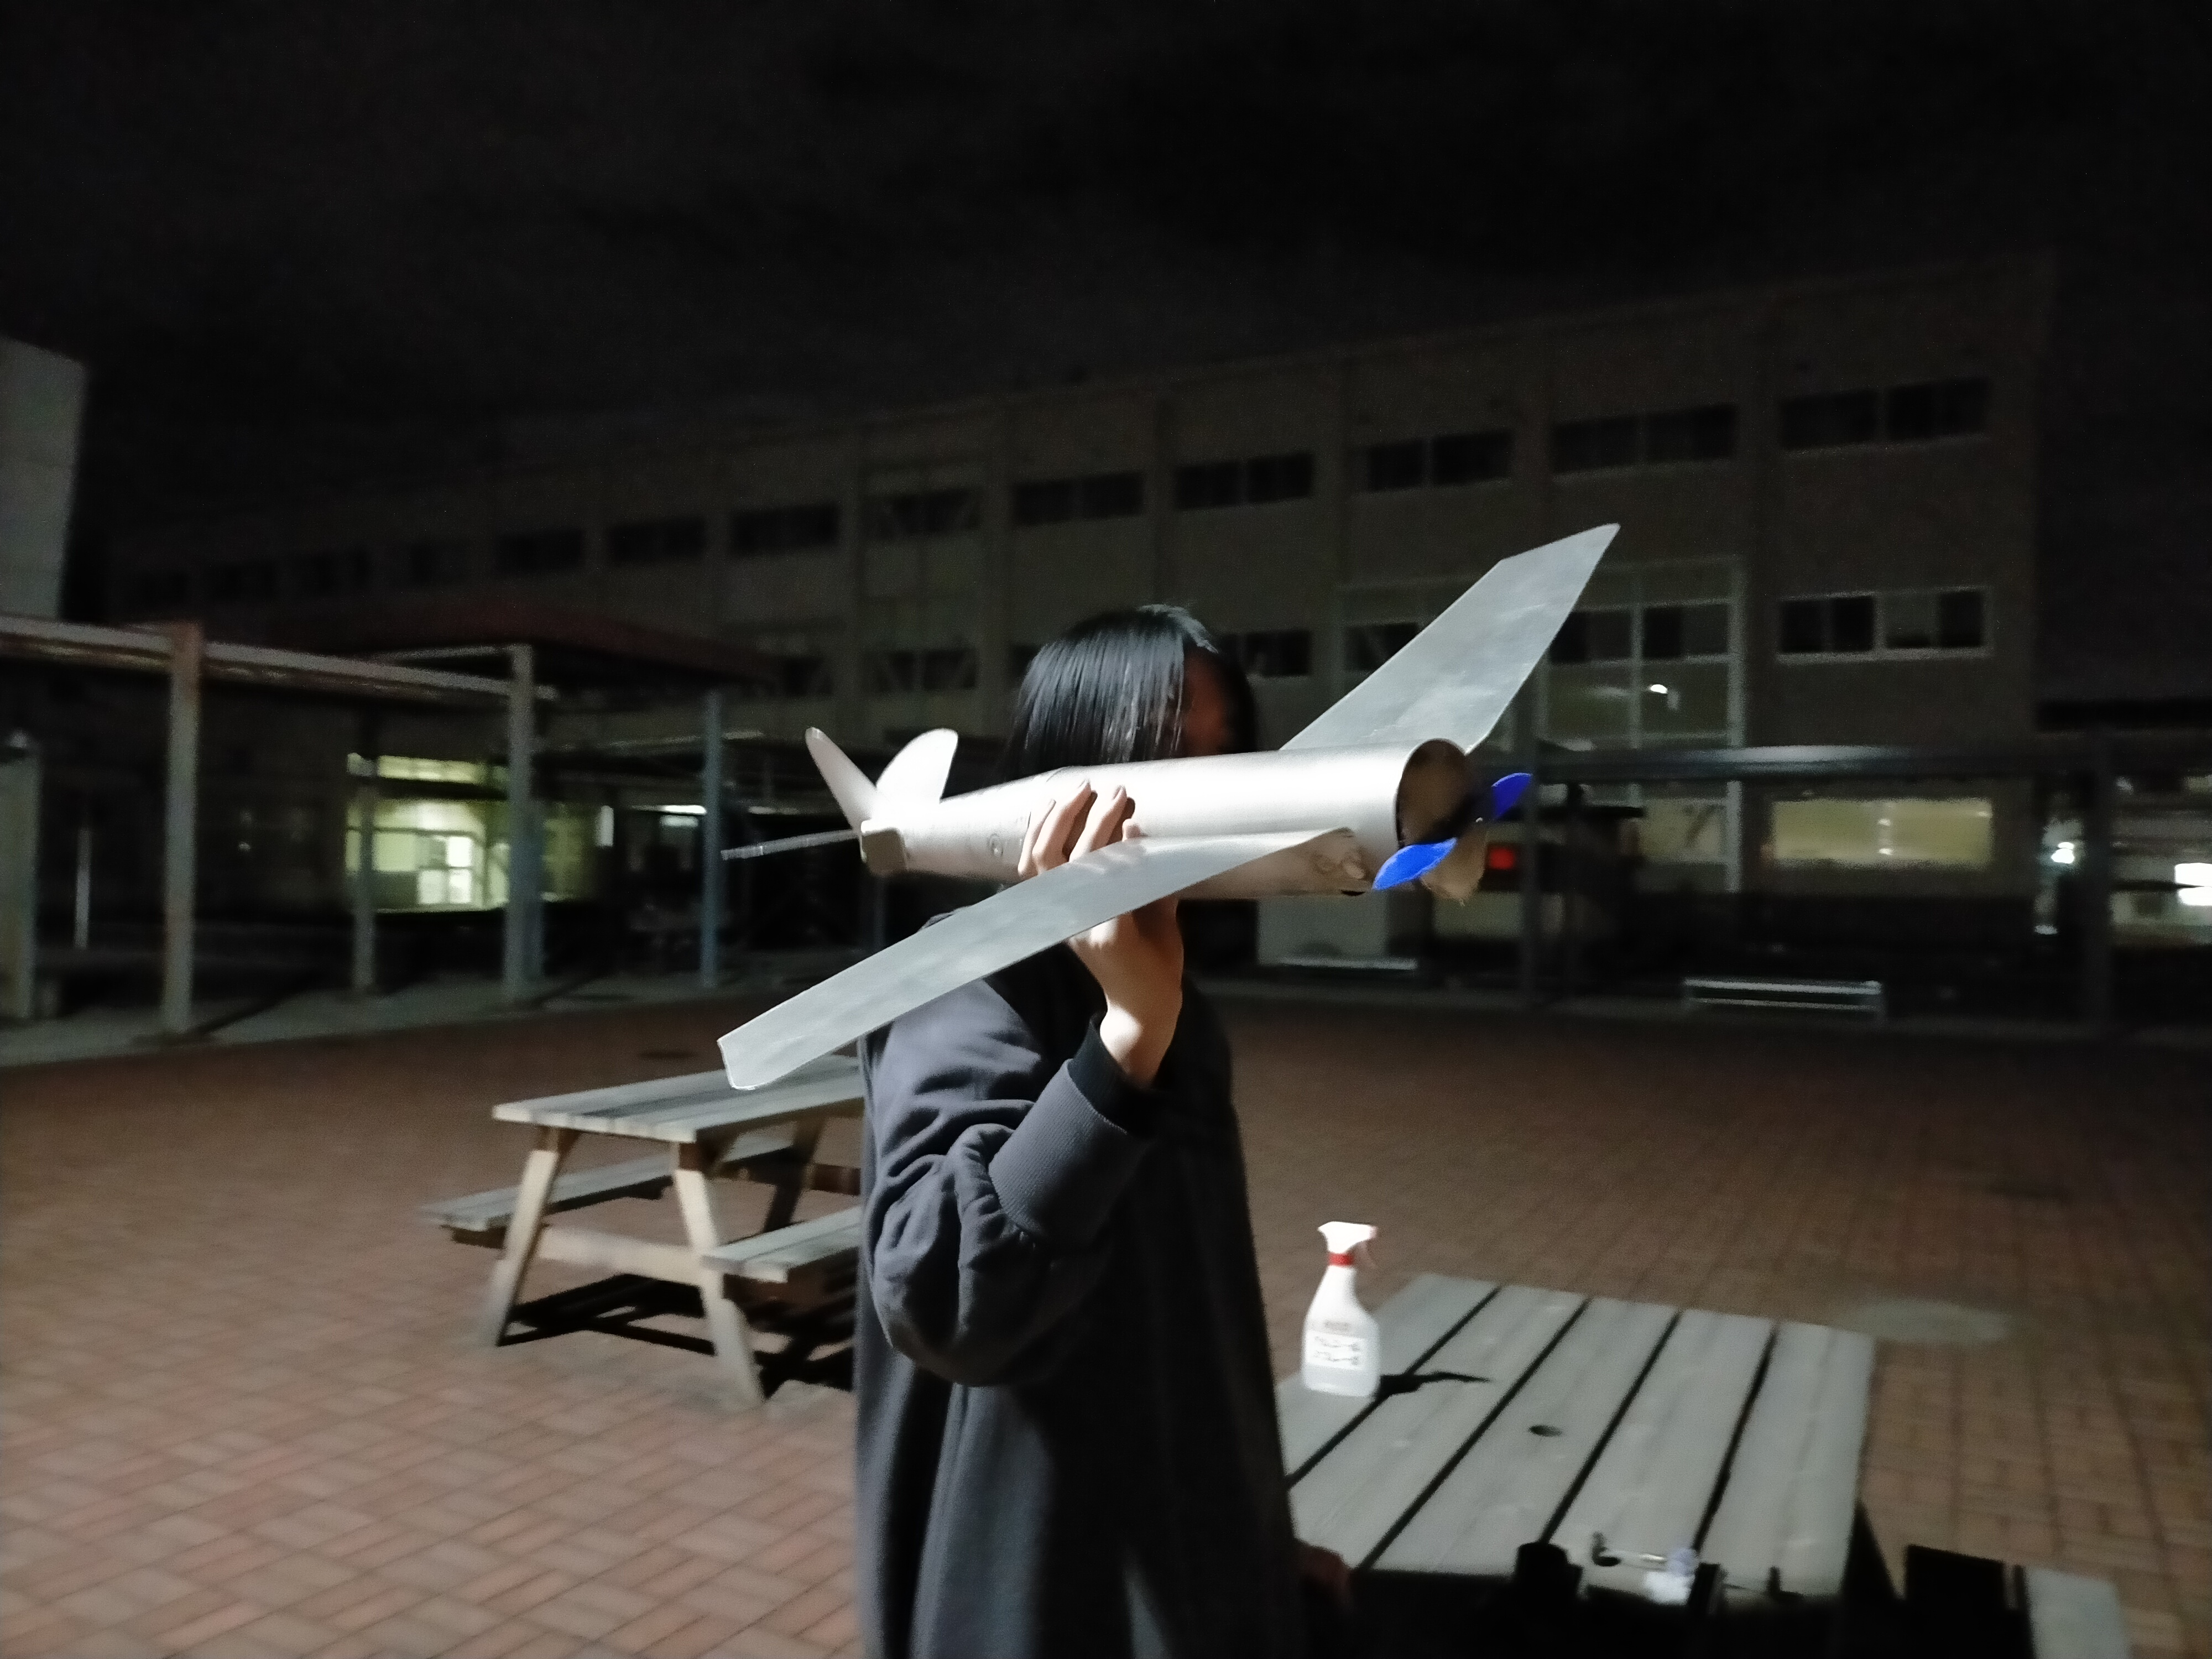
\includegraphics[scale=.02]{pic/mecafe3.jpg}
          \end{center}
        \end{alertblock}
      \end{footnotesize}
    \end{column}
    \begin{column}{.3\textwidth}
      \begin{footnotesize}
        \begin{alertblock}{\normalsize 金属3Dプリント}
          \begin{center}
            金属の3Dプリンターで\\
            様々なモノを製作\\
            \includegraphics[scale=.02,angle=-90]{pic/mecafe2.jpg}
          \end{center}
        \end{alertblock}
      \end{footnotesize}
    \end{column}
  \end{columns}

  \begin{textblock*}{0.4\linewidth}(300pt,5pt)
    \begin{tikzpicture}[scale=.8]
      %座標設定
      \coordinate (A) at (0,-.1);
      \coordinate (B) at (0,1);
      \coordinate (C) at ({cos(9*pi/10 r)},{sin(9*pi/10 r)});
      \coordinate (D) at ({cos(13*pi/10 r)},{sin(13*pi/10 r)});
      \coordinate (E) at ({cos(17*pi/10 r)},{sin(17*pi/10 r)});
      \coordinate (F) at ({cos(21*pi/10 r)},{sin(21*pi/10 r)});
      %線引き
      \draw[line width = 2pt] (F)--(B)--(C)--(D)--(E)--cycle;
      %nodeのスタイル指定
      \tikzset{block/.style={circle,white,fill=cyan,minimum size=.65cm,inner sep=0pt}};
      %node(テキストボックス的な)を指定座標に配置
      \node[inner sep=0pt] at (A) {\includegraphics[width=.7cm]{pic/Logo.png}};
      \node[block,fill=LightUIRed] at (B) {\tiny MeCafe};
      \node[block] at (C) {\tiny メカ研};
      \node[block] at (D) {\tiny 電研};
      \node[block] at (E) {\tiny シス研};
      \node[block] at (F) {\tiny 情研};
    \end{tikzpicture}
  \end{textblock*}
\end{frame}

\begin{frame}{TechRingを創る仲間たち その2}{機械研究会}

  \vspace{-2mm}
  
  \begin{minipage}{0.85\textwidth}
    \begin{block}{活動内容}
      \begin{itemize}
        \item Nゲージジオラマの製作
        \item HOゲージ車両の作成
      \end{itemize}
    \end{block}
  \end{minipage}

  \begin{alertblock}{京都天橋立 ジオラマ}
    \begin{columns}[totalwidth=\textwidth]
      \begin{column}{0.5\textwidth}
        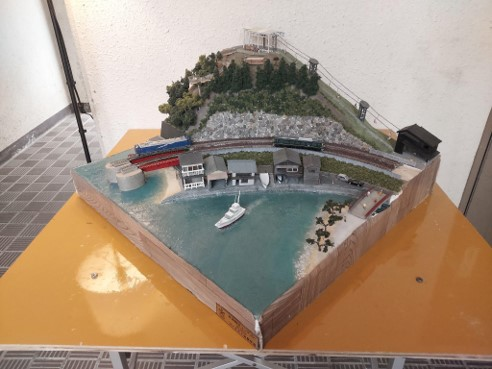
\includegraphics[scale=0.42]{pic/mekaken1.jpg}
      \end{column}
      \begin{column}{0.22\textwidth}
        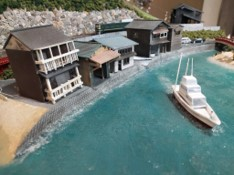
\includegraphics[scale=0.4]{pic/mekaken2.jpg}\\
        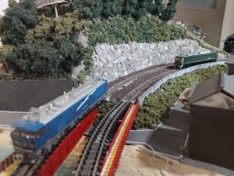
\includegraphics[scale=0.4]{pic/mekaken3.jpg}
      \end{column}
      \begin{column}{0.25\textwidth}
        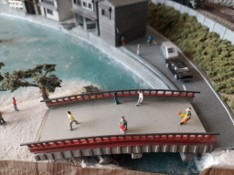
\includegraphics[scale=0.4]{pic/mekaken4.jpg}\\
        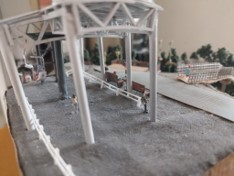
\includegraphics[scale=0.4]{pic/mekaken5.jpg}
      \end{column}
    \end{columns}
  \end{alertblock}

  \begin{textblock*}{0.4\linewidth}(300pt,5pt)
    \begin{tikzpicture}[scale=.8]
      %座標設定
      \coordinate (A) at (0,-.1);
      \coordinate (B) at (0,1);
      \coordinate (C) at ({cos(9*pi/10 r)},{sin(9*pi/10 r)});
      \coordinate (D) at ({cos(13*pi/10 r)},{sin(13*pi/10 r)});
      \coordinate (E) at ({cos(17*pi/10 r)},{sin(17*pi/10 r)});
      \coordinate (F) at ({cos(21*pi/10 r)},{sin(21*pi/10 r)});
      %線引き
      \draw[line width = 2pt] (F)--(B)--(C)--(D)--(E)--cycle;
      %nodeのスタイル指定
      \tikzset{block/.style={circle,white,fill=cyan,minimum size=.65cm,inner sep=0pt}};
      %node(テキストボックス的な)を指定座標に配置
      \node[inner sep=0pt] at (A) {\includegraphics[width=.7cm]{pic/Logo.png}};
      \node[block] at (B) {\tiny MeCafe};
      \node[block,fill=LightUIRed] at (C) {\tiny メカ研};
      \node[block] at (D) {\tiny 電研};
      \node[block] at (E) {\tiny シス研};
      \node[block] at (F) {\tiny 情研};
    \end{tikzpicture}
  \end{textblock*}
\end{frame}

\begin{frame}{TechRingを創る仲間たち その3}{電気技術研究会}

  \vspace{-2mm}
  
  \begin{minipage}{0.85\textwidth}
    \begin{block}{活動内容}
      \begin{itemize}
        \item 高専祭展示品製作
        \item 各種コンテストの参加
        \item 電子工作から衛星の電波受信まで幅広く活動
      \end{itemize}
    \end{block}
  \end{minipage}

  \vspace{-2mm}

  \begin{columns}[totalwidth=\textwidth]
    \begin{column}{.48\textwidth}
      \begin{footnotesize}
        \begin{alertblock}{\normalsize Ele Mag Harmony}
            \begin{center}
              ソレノイドやステッピングモータ\\
              FDDやリレーで音楽を演奏\\
            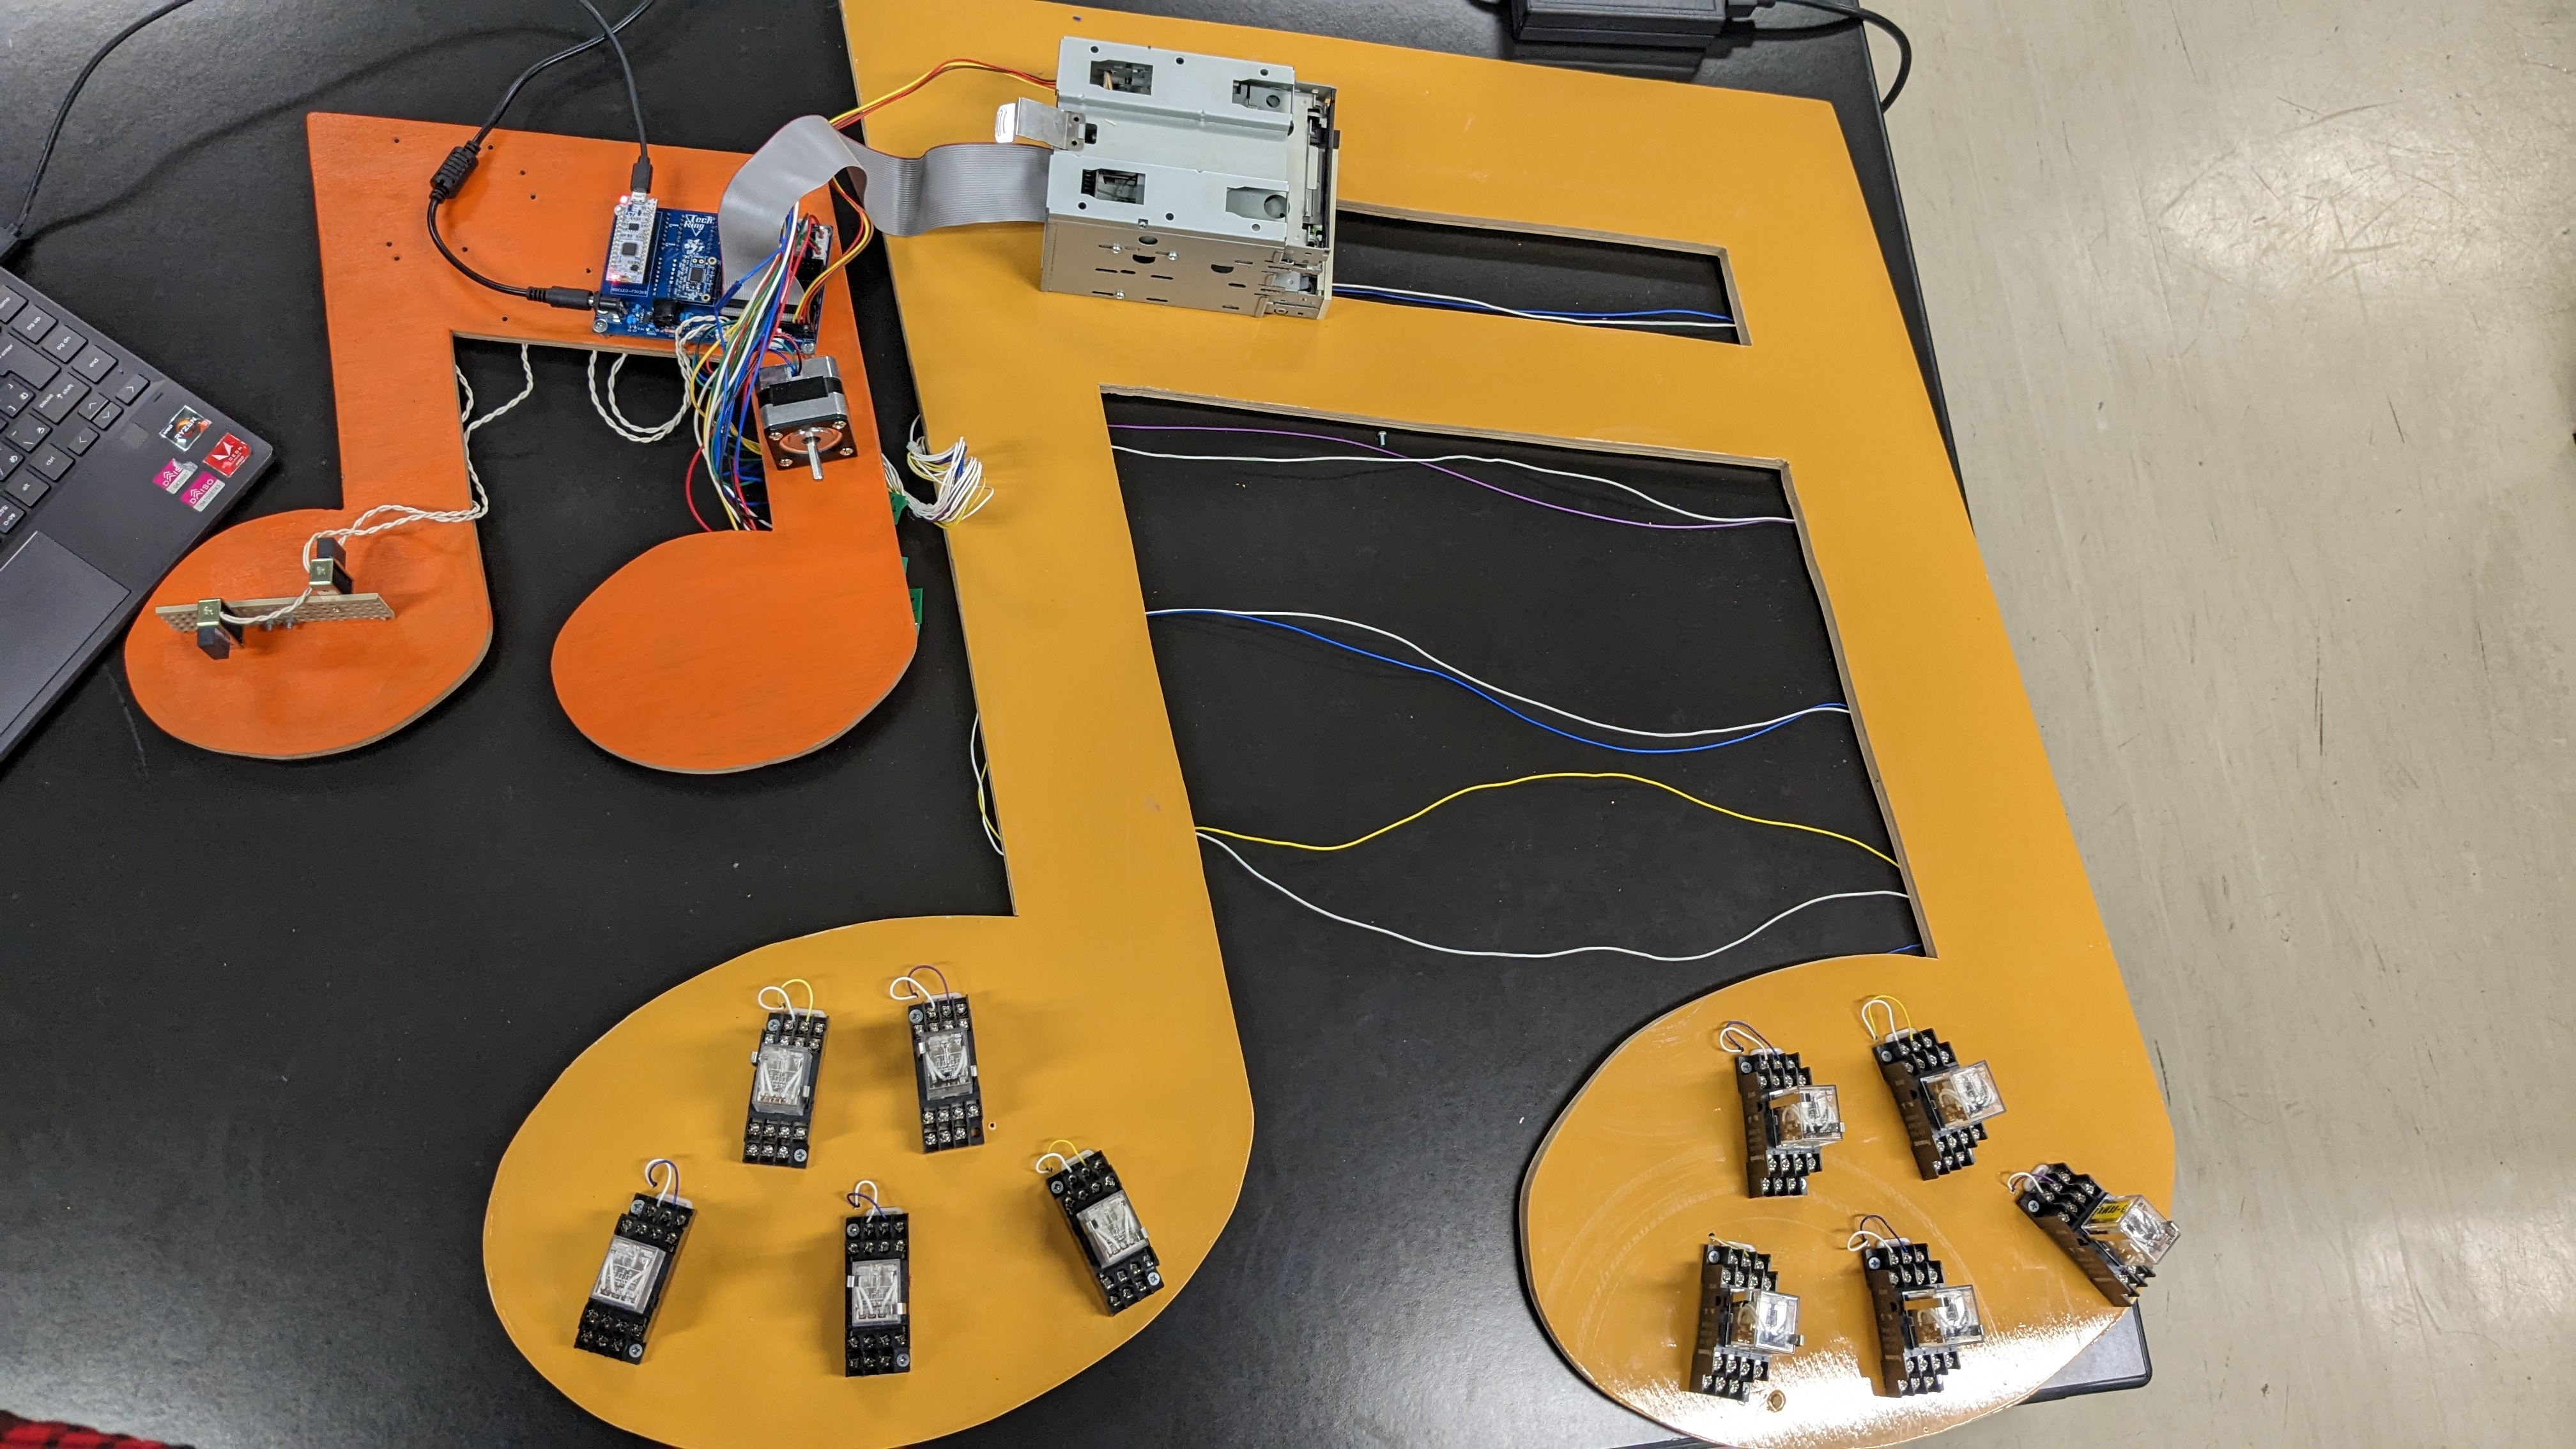
\includegraphics[scale=.035]{pic/denken1.jpg}
            \end{center}
        \end{alertblock}
      \end{footnotesize}
    \end{column}
    \begin{column}{.48\textwidth}
      \begin{footnotesize}
        \begin{alertblock}{\normalsize Nixie Clock \& LED Matrix}
          \begin{center}
            ニキシー管で時計を製作\\
            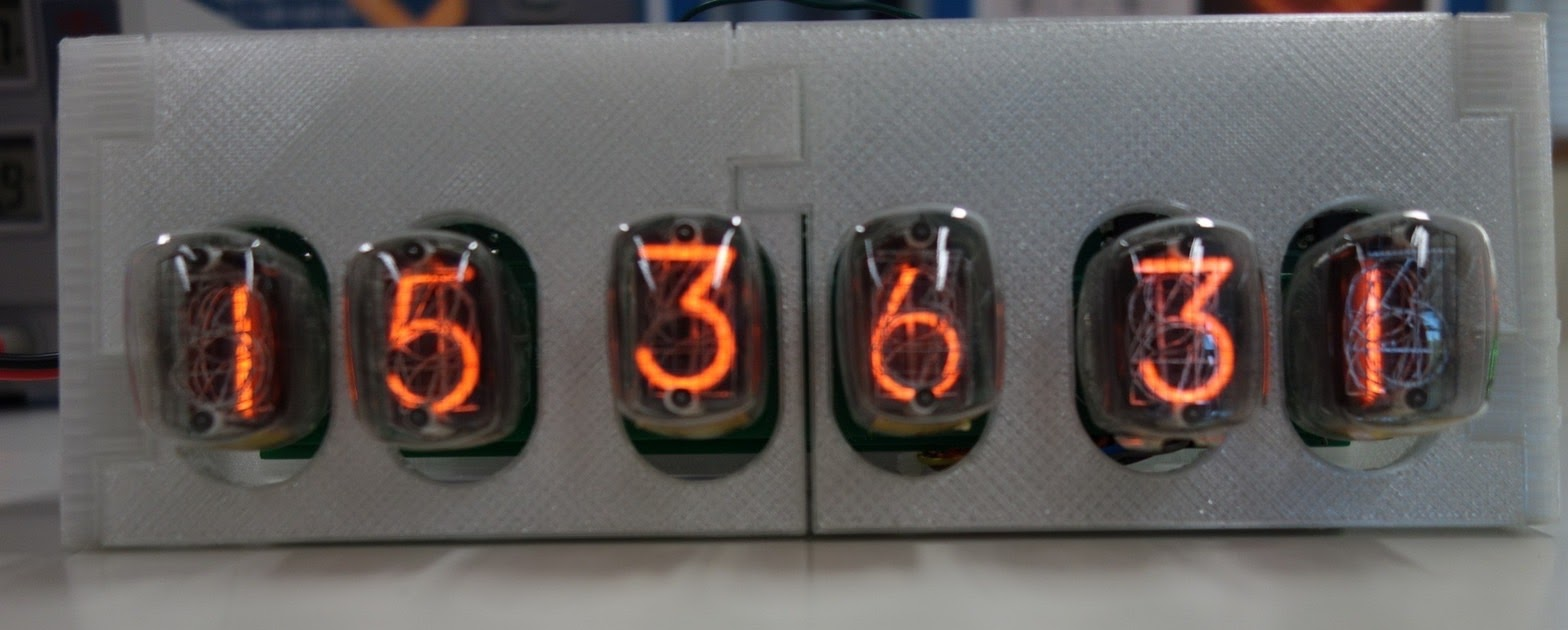
\includegraphics[scale=.06]{pic/denken2.jpg}\\
            LED Matrixでアニメーション\\
            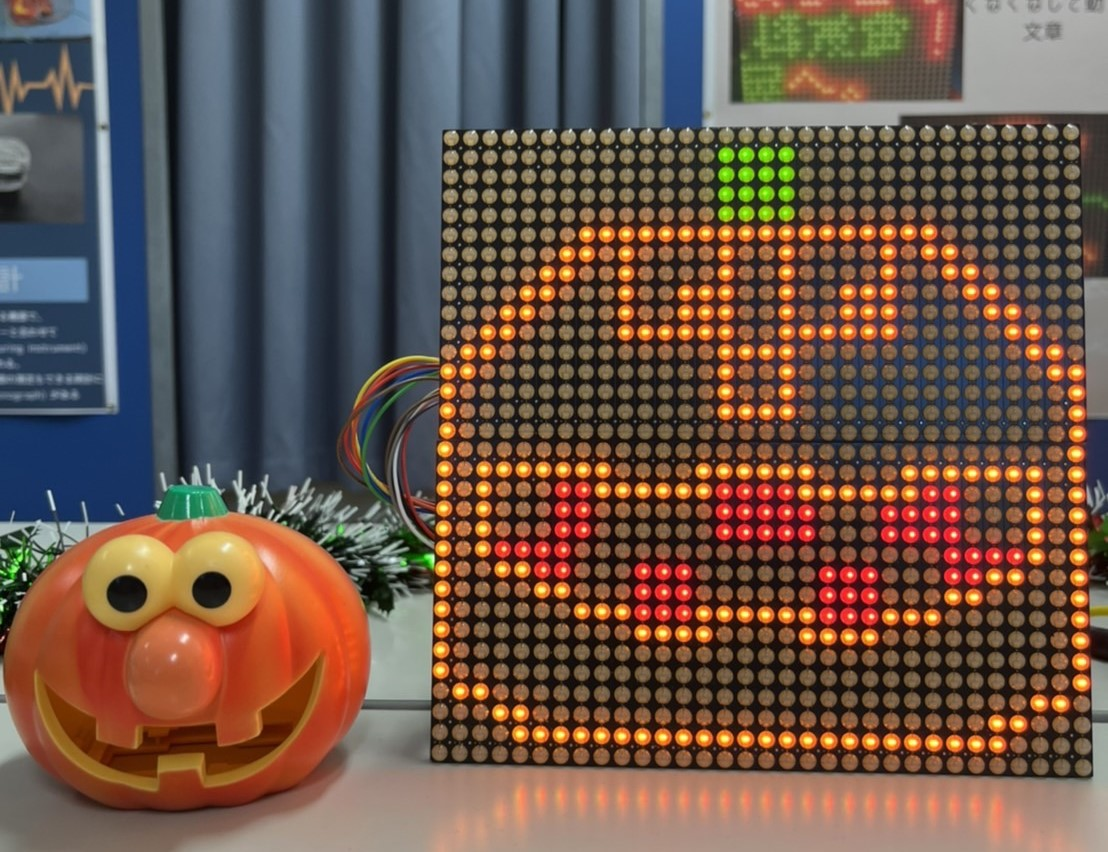
\includegraphics[scale=.08]{pic/denken3.jpg}
          \end{center}
        \end{alertblock}
      \end{footnotesize}
    \end{column}
  \end{columns}

  \begin{textblock*}{0.4\linewidth}(300pt,5pt)
    \begin{tikzpicture}[scale=.8]
      %座標設定
      \coordinate (A) at (0,-.1);
      \coordinate (B) at (0,1);
      \coordinate (C) at ({cos(9*pi/10 r)},{sin(9*pi/10 r)});
      \coordinate (D) at ({cos(13*pi/10 r)},{sin(13*pi/10 r)});
      \coordinate (E) at ({cos(17*pi/10 r)},{sin(17*pi/10 r)});
      \coordinate (F) at ({cos(21*pi/10 r)},{sin(21*pi/10 r)});
      %線引き
      \draw[line width = 2pt] (F)--(B)--(C)--(D)--(E)--cycle;
      %nodeのスタイル指定
      \tikzset{block/.style={circle,white,fill=cyan,minimum size=.65cm,inner sep=0pt}};
      %node(テキストボックス的な)を指定座標に配置
      \node[inner sep=0pt] at (A) {\includegraphics[width=.7cm]{pic/Logo.png}};
      \node[block] at (B) {\tiny MeCafe};
      \node[block] at (C) {\tiny メカ研};
      \node[block,fill=LightUIRed] at (D) {\tiny 電研};
      \node[block] at (E) {\tiny シス研};
      \node[block] at (F) {\tiny 情研};
    \end{tikzpicture}
  \end{textblock*}
\end{frame}

\begin{frame}{TechRingを創る仲間たち その4}{システム開発研究会}
  
  \vspace{-2mm}
  
  \begin{minipage}{0.85\textwidth}
    \begin{block}{活動内容}
      \begin{itemize}
        \item 興味関心を深め知識技術を身に着ける!
        \item 高専祭での展示
        \item 小中学生向けロボット教室
        \item WRO(LEGOによるロボコン)
        \item 地域との共同企画
      \end{itemize}
    \end{block}
  \end{minipage}

  \begin{footnotesize}
    \begin{columns}[T,totalwidth=1.01\textwidth]
      \begin{column}{.20\textwidth}
        \begin{center}
          \alert{モデリング}\\
          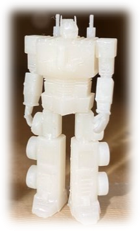
\includegraphics[scale=0.5]{pic/shisuken1.png}
        \end{center}
      \end{column}
      \begin{column}{.20\textwidth}
        \begin{center}
          \alert{ロボット}\\
          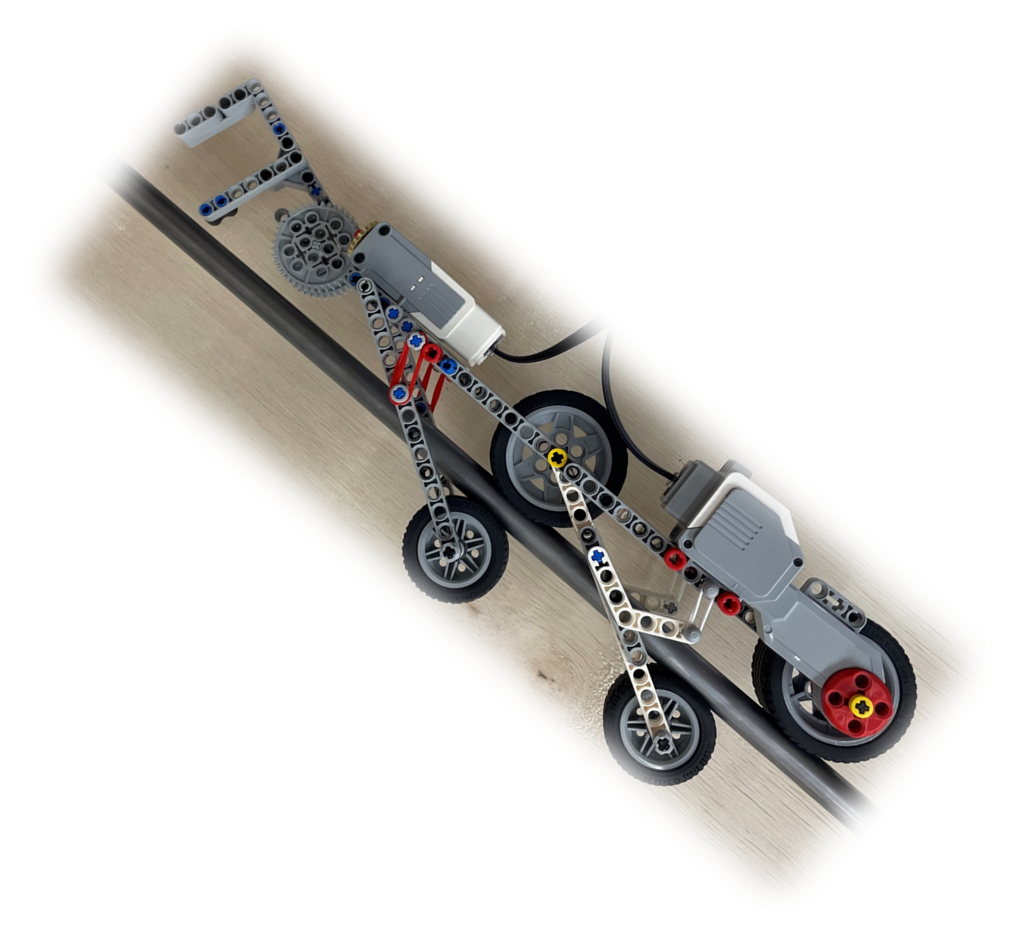
\includegraphics[scale=0.5,angle=30]{pic/shisuken2.png}
        \end{center}
      \end{column}
      \begin{column}{.20\textwidth}
        \begin{center}
          \alert{電子工作}\\
          \vspace{1mm}
          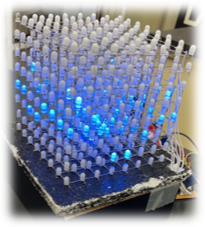
\includegraphics[scale=0.4]{pic/shisuken3.png}
        \end{center}
      \end{column}
      \begin{column}{.20\textwidth}
        \begin{center}
          \alert{プログラミング}\\
          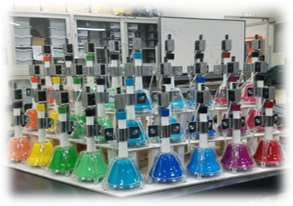
\includegraphics[scale=0.3]{pic/shisuken5.png}
        \end{center}
      \end{column}
      \begin{column}{.20\textwidth}
        \begin{center}
          \alert{3Dプリンタ}\\
          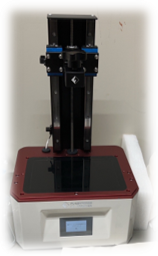
\includegraphics[scale=0.45]{pic/shisuken4.png}
        \end{center}
      \end{column}
    \end{columns}
  \end{footnotesize}

  \begin{textblock*}{0.4\linewidth}(300pt,5pt)
    \begin{tikzpicture}[scale=.8]
      %座標設定
      \coordinate (A) at (0,-.1);
      \coordinate (B) at (0,1);
      \coordinate (C) at ({cos(9*pi/10 r)},{sin(9*pi/10 r)});
      \coordinate (D) at ({cos(13*pi/10 r)},{sin(13*pi/10 r)});
      \coordinate (E) at ({cos(17*pi/10 r)},{sin(17*pi/10 r)});
      \coordinate (F) at ({cos(21*pi/10 r)},{sin(21*pi/10 r)});
      %線引き
      \draw[line width = 2pt] (F)--(B)--(C)--(D)--(E)--cycle;
      %nodeのスタイル指定
      \tikzset{block/.style={circle,white,fill=cyan,minimum size=.65cm,inner sep=0pt}};
      %node(テキストボックス的な)を指定座標に配置
      \node[inner sep=0pt] at (A) {\includegraphics[width=.7cm]{pic/Logo.png}};
      \node[block] at (B) {\tiny MeCafe};
      \node[block] at (C) {\tiny メカ研};
      \node[block] at (D) {\tiny 電研};
      \node[block,fill=LightUIRed] at (E) {\tiny シス研};
      \node[block] at (F) {\tiny 情研};
    \end{tikzpicture}
  \end{textblock*}
\end{frame}

\begin{frame}{TechRingを創る仲間たち その5}{情報処理研究会}
  
  \vspace{-2mm}

  \begin{columns}[totalwidth=\textwidth]
    \begin{column}{0.4\textwidth}
      \begin{block}{活動内容}
        \begin{itemize}
          \item 各種コンテスト参加
          \item 講習会の実施
          \item 自作PCの組み立て
        \end{itemize}
      \end{block}
    \end{column}
    \begin{column}{0.5\textwidth}
      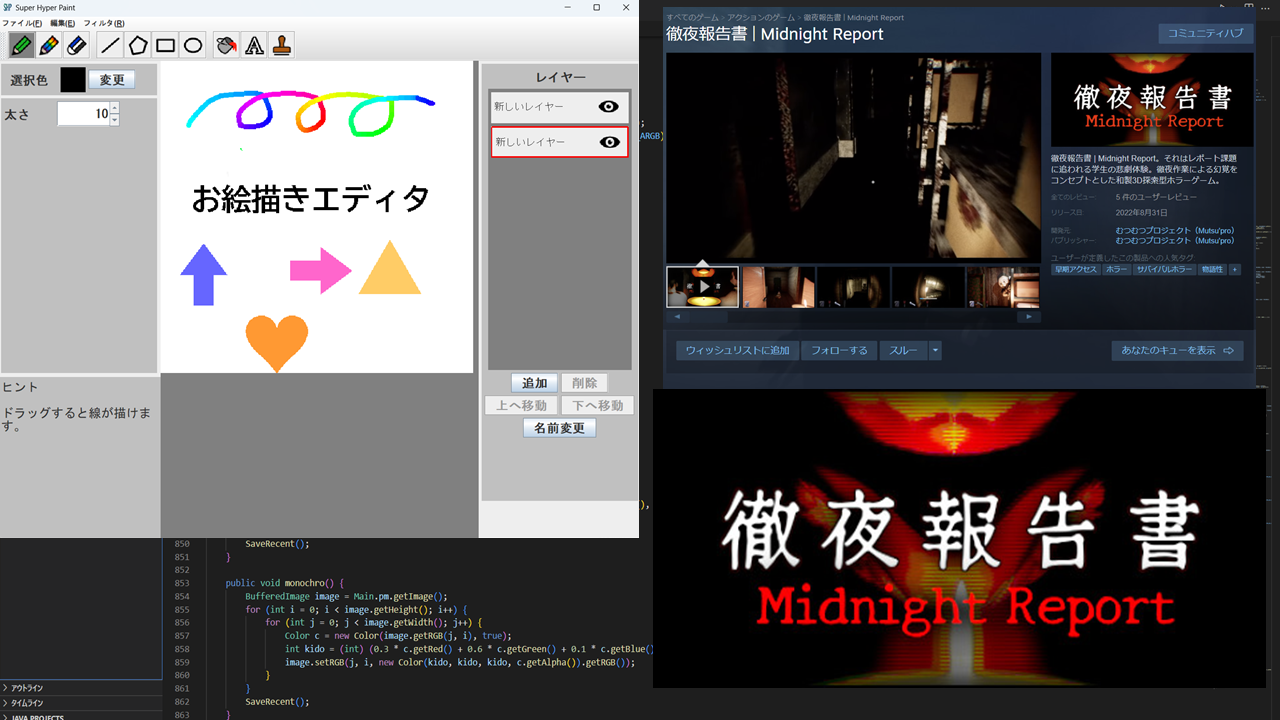
\includegraphics[scale=.13]{pic/joken.png}
    \end{column}
  \end{columns}

  \vspace{-2mm}

  \begin{columns}
    \begin{column}{0.48\textwidth}
      \begin{alertblock}{Super Hyper Paint}
        \begin{footnotesize}
          \begin{description}
            \item[使用言語] Java
            \item[機能] ファイルの作成\\読み込み 保存\\上書き保存 図形\\
            元に戻す 色反転\\白黒化 虹色ペン\\消しゴム 色の選択\\塗りつぶし 文字入力\\レイヤー機能 ヒント
          \end{description}
        \end{footnotesize}
      \end{alertblock}
    \end{column}
    \begin{column}{0.48\textwidth}
      \begin{alertblock}{徹夜報告書|Midnight Report}
        \begin{footnotesize}
          \begin{description}[ゲームエンジン]
            \item[ゲームエンジン] UE4 v4.26
            \item[モデリング] Blender
            \item[画像処理] Gimp
            \item[音声作成] GarageBand 
          \end{description}
          \begin{itemize}
            \item 素材のほぼすべてを独自で制作
            \item Steamにて販売
            \item あのガッチマンもプレイした!?
          \end{itemize}
        \end{footnotesize}
      \end{alertblock}
    \end{column}
  \end{columns}

  \begin{textblock*}{0.4\linewidth}(300pt,5pt)
    \begin{tikzpicture}[scale=.8]
      %座標設定
      \coordinate (A) at (0,-.1);
      \coordinate (B) at (0,1);
      \coordinate (C) at ({cos(9*pi/10 r)},{sin(9*pi/10 r)});
      \coordinate (D) at ({cos(13*pi/10 r)},{sin(13*pi/10 r)});
      \coordinate (E) at ({cos(17*pi/10 r)},{sin(17*pi/10 r)});
      \coordinate (F) at ({cos(21*pi/10 r)},{sin(21*pi/10 r)});
      %線引き
      \draw[line width = 2pt] (F)--(B)--(C)--(D)--(E)--cycle;
      %nodeのスタイル指定
      \tikzset{block/.style={circle,white,fill=cyan,minimum size=.65cm,inner sep=0pt}};
      %node(テキストボックス的な)を指定座標に配置
      \node[inner sep=0pt] at (A) {\includegraphics[width=.7cm]{pic/Logo.png}};
      \node[block] at (B) {\tiny MeCafe};
      \node[block] at (C) {\tiny メカ研};
      \node[block] at (D) {\tiny 電研};
      \node[block] at (E) {\tiny シス研};
      \node[block,fill=LightUIRed] at (F) {\tiny 情研};
    \end{tikzpicture}
  \end{textblock*}
\end{frame}

\begin{frame}{TechRingのこれから}{アッと驚く技術を、もっと広く世界へ}
  \begin{tikzpicture}[overlay]
    \node at (9, 1){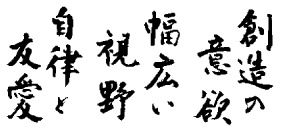
\includegraphics[scale=.3]{pic/kyoiku.jpg}};
  \end{tikzpicture}

  \vspace{-5mm}

  \begin{block}{大高専時代へ}
    \vspace{2mm}
    \begin{description}
      \setlength{\itemsep}{2mm}
      \item[創造の意欲] 学内イベントの開催により\\
      創作活動のモチベーションを上げ、活発化を目指す
      \item[幅広い視野] 学外への技術発信を行い\\
      アウトプットからフィードバックを得る
      \item[自律と友愛] チーム開発の経験から\\
      仲間とのコミュニケーションの重要さを学ぶ
    \end{description}
  \end{block}

  \vfill

  \begin{Large}
    モノを作るだけではなく \vfill \hspace{7em}\alert{コトを起こす}ものづくりを
  \end{Large}
\end{frame}

\begin{frame}[plain,noframenumbering]
  \begin{center}
    \begin{Large}
      ご清聴、ありがとうございました。
    \end{Large}
  \end{center}

  \begin{alertblock}{Follow me}
    \begin{center}
      ブース展示 G-03-04\\
      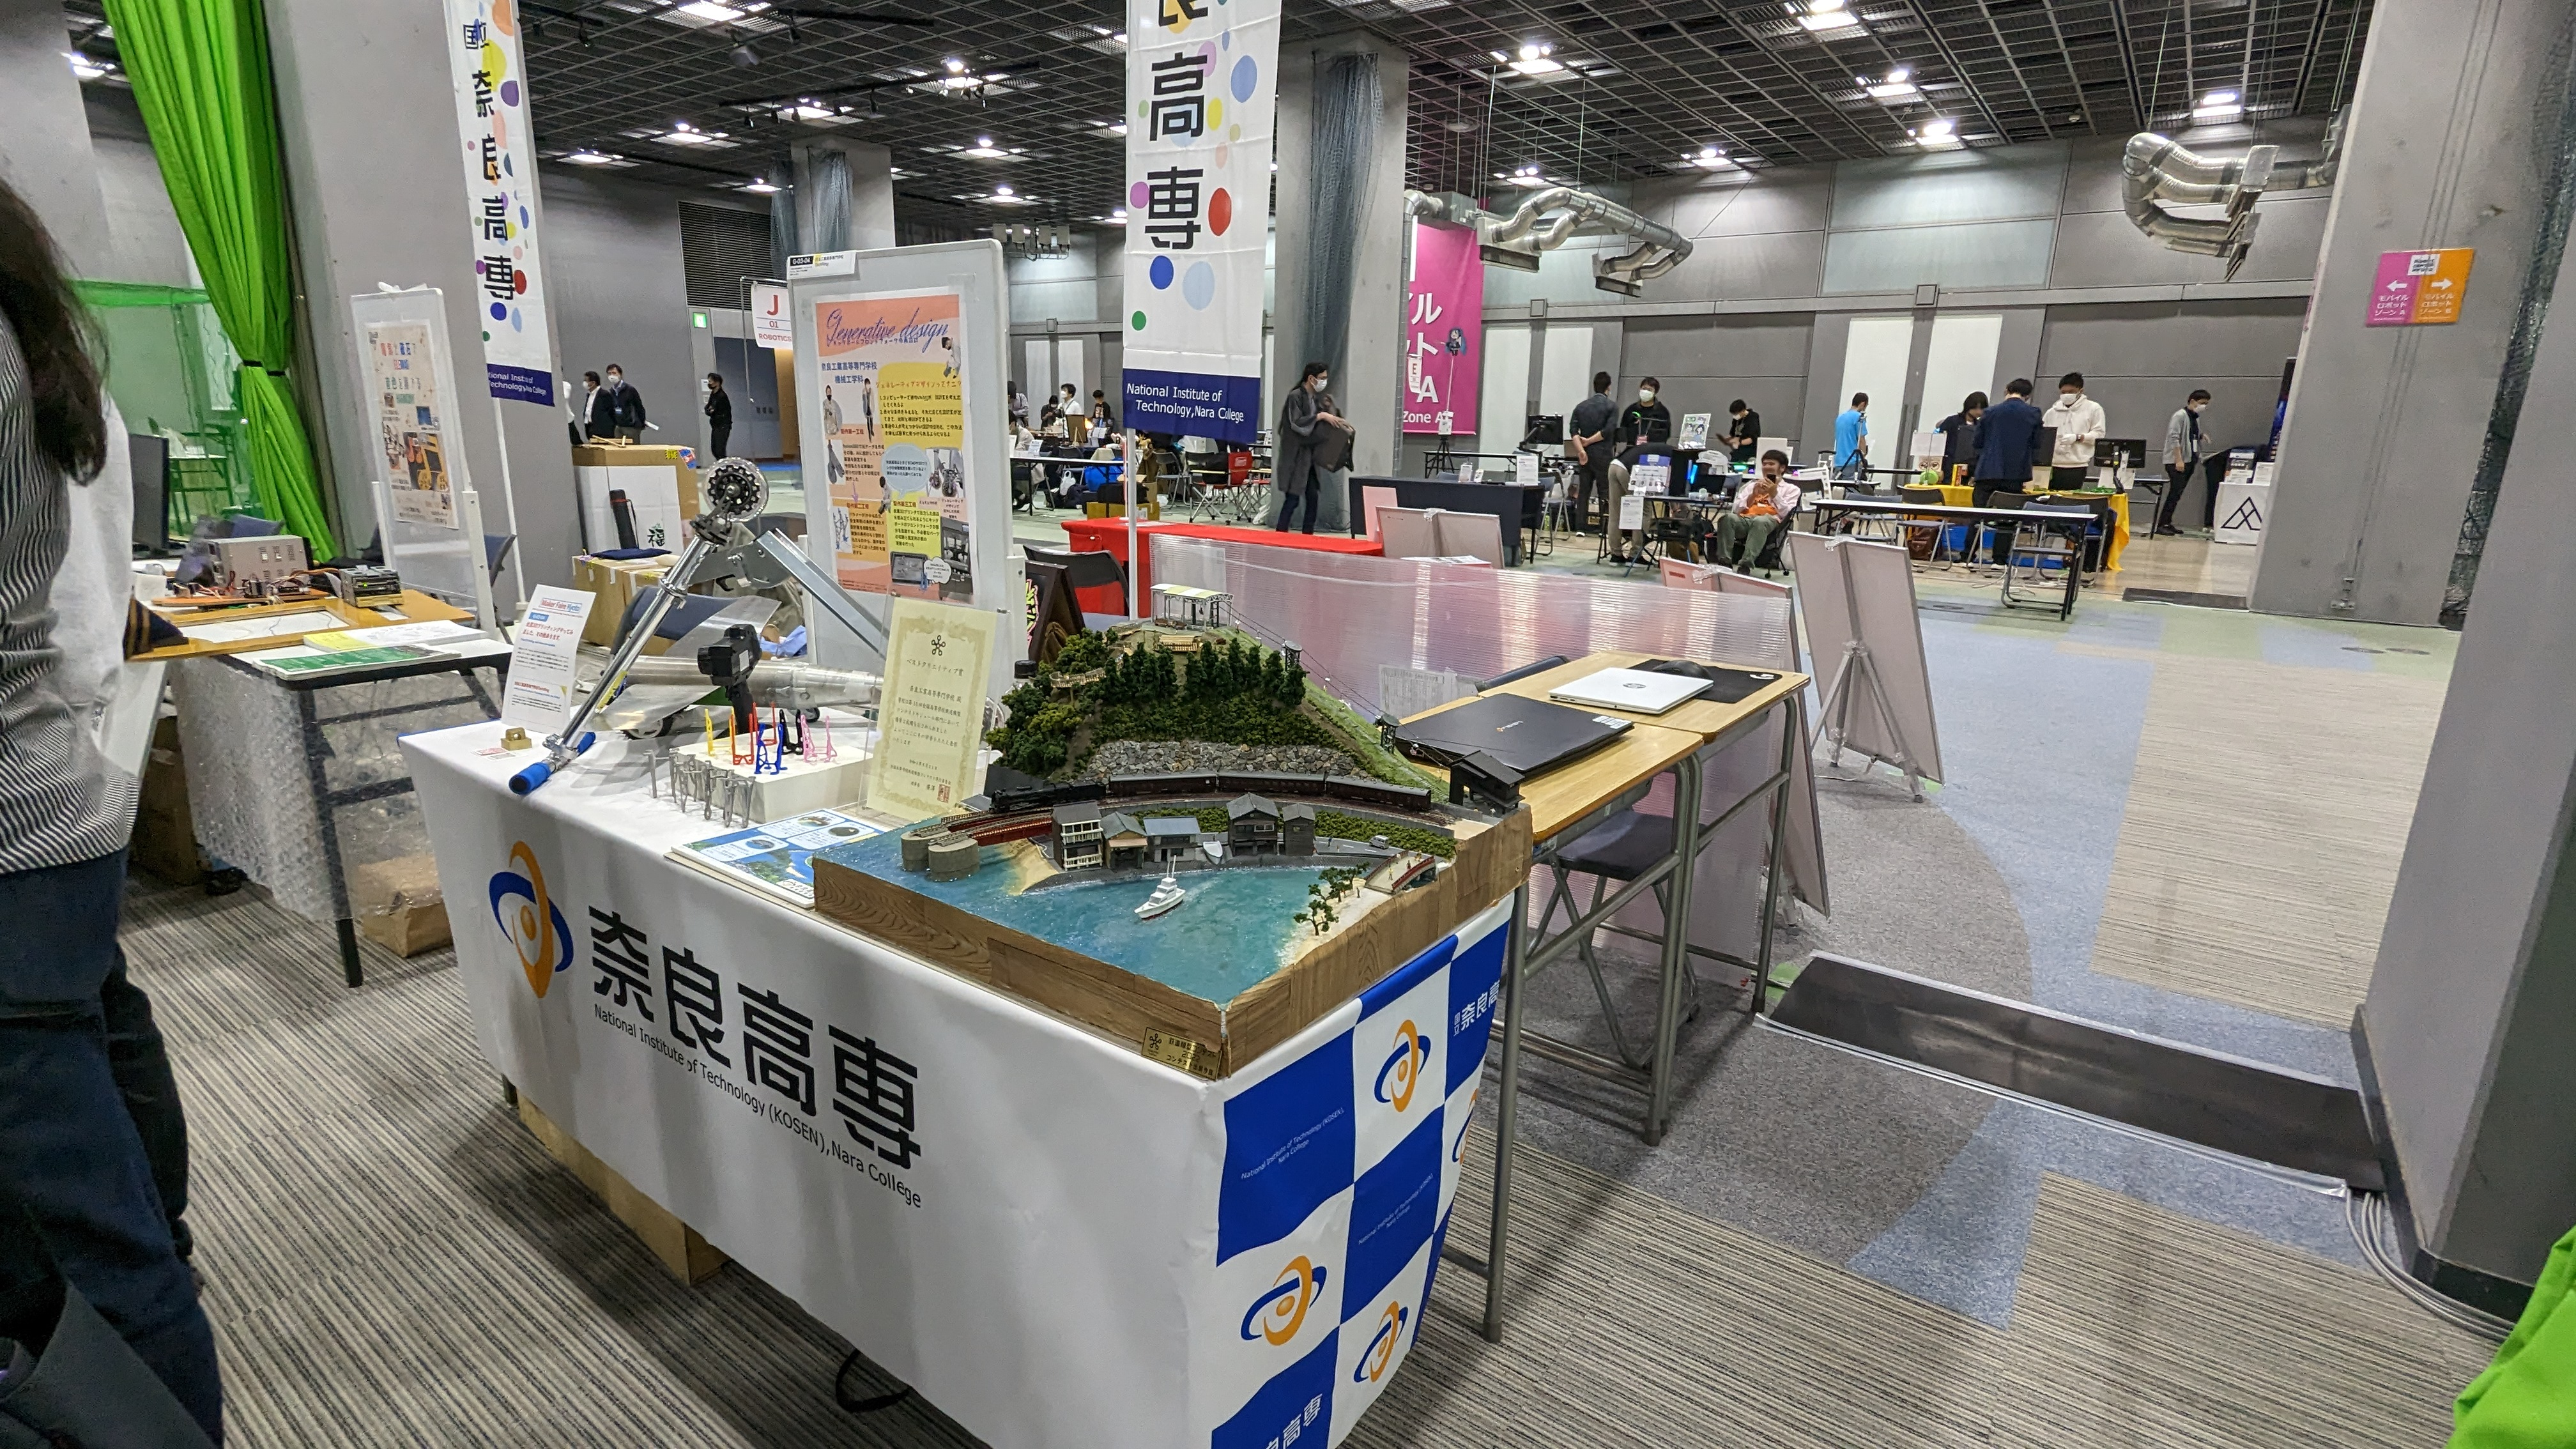
\includegraphics[width=0.36\textwidth]{pic/Booth.jpg}\\
      公式Twitter\\
      
\includegraphics[width=0.24\textwidth]{pic/Twitter.png}
    \end{center}
  \end{alertblock}
\end{frame}

\end{document}